% !TeX program = xelatex
% !TeX encoding = UTF-8
\documentclass[12pt,openany,oneside]{book}

% -----------------------------------------------------------------------------
% Page, mathematics, tables, graphics
% -----------------------------------------------------------------------------
\usepackage[a4paper,top=23mm,bottom=25mm,left=25mm,right=25mm,headheight=17pt]{geometry}
\usepackage{amsmath,amssymb,amsfonts,mathtools,bm}
\usepackage{amsthm}
\usepackage{booktabs,longtable,array,multirow,tabularx}
\usepackage{graphicx}
\graphicspath{{figures/}}
\usepackage{xcolor}
\usepackage{tikz}
\usetikzlibrary{arrows.meta,positioning,calc,fit,shapes.geometric,decorations.pathreplacing,matrix,patterns,3d}
\usepackage[most]{tcolorbox}
\usepackage{enumitem}
\usepackage{listings}
\usepackage{caption}
\usepackage{subcaption}
\usepackage{float}
\usepackage{fancyhdr}
\usepackage{titlesec}
\usepackage{setspace}
\usepackage{microtype}
\usepackage{hyperref}
\usepackage{xepersian}

% -----------------------------------------------------------------------------
% Robust font configuration: same convention as Chapters 2--5
% -----------------------------------------------------------------------------
\IfFontExistsTF{Amiri}
  {\settextfont[Scale=1.08]{Amiri}\setdigitfont{Amiri}}
  {\settextfont[Scale=1.05]{Noto Naskh Arabic}\setdigitfont{Noto Naskh Arabic}}
\IfFontExistsTF{DejaVu Serif}
  {\setlatintextfont{DejaVu Serif}}
  {\setlatintextfont{Latin Modern Roman}}
\IfFontExistsTF{DejaVu Sans Mono}
  {\setmonofont{DejaVu Sans Mono}}
  {\setmonofont{Latin Modern Mono}}

% -----------------------------------------------------------------------------
% Visual identity
% -----------------------------------------------------------------------------
\definecolor{DeepBlue}{HTML}{163A5F}
\definecolor{Accent}{HTML}{B34B35}
\definecolor{SoftBlue}{HTML}{EAF2F8}
\definecolor{SoftGold}{HTML}{FFF6DF}
\definecolor{SoftGreen}{HTML}{EAF7EF}
\definecolor{SoftRed}{HTML}{FCEDEC}
\definecolor{SoftGray}{HTML}{F4F5F6}
\definecolor{CodeGray}{HTML}{F7F7F7}

\hypersetup{
  colorlinks=true,
  linkcolor=DeepBlue,
  citecolor=Accent,
  urlcolor=Accent,
  pdftitle={پردازش تصویر در دهه آینده ـ فصل هفتم: ساختار محلی و مورفولوژی},
  pdfauthor={جزوه درس کارشناسی ارشد}
}

\setstretch{1.22}
\setlength{\parskip}{0.35em}
\setlength{\parindent}{1.3em}
\setlist[itemize]{itemsep=0.25em,topsep=0.35em,leftmargin=9mm}
\setlist[enumerate]{itemsep=0.25em,topsep=0.35em,leftmargin=10mm}

\pagestyle{fancy}
\fancyhf{}
\fancyhead[R]{\small\thepage}
\fancyhead[L]{\small\nouppercase{\leftmark}}
\renewcommand{\headrulewidth}{0.4pt}

\titleformat{\chapter}[display]
  {\normalfont\huge\bfseries\color{DeepBlue}}
  {\filleft\Large فصل \thechapter}
  {8pt}
  {\filright}
\titleformat{\section}{\Large\bfseries\color{DeepBlue}}{\thesection}{0.7em}{}
\titleformat{\subsection}{\large\bfseries\color{Accent}}{\thesubsection}{0.7em}{}
\titleformat{\subsubsection}{\normalsize\bfseries\color{DeepBlue}}{\thesubsubsection}{0.7em}{}

% -----------------------------------------------------------------------------
% Theorems and boxes
% -----------------------------------------------------------------------------
\newtheorem{definition}{تعریف}[chapter]
\newtheorem{theorem}{قضیه}[chapter]
\newtheorem{proposition}{گزاره}[chapter]
\newtheorem{lemma}{لم}[chapter]
\newtheorem{example}{مثال}[chapter]
\newtheorem{remark}{نکته}[chapter]
\newtheorem{corollary}{نتیجه}[chapter]
\renewcommand{\proofname}{اثبات}

\newtcolorbox{learningbox}{colback=SoftBlue,colframe=DeepBlue,title=اهداف یادگیری,fonttitle=\bfseries,breakable,enhanced}
\newtcolorbox{keybox}[1][]{colback=SoftGold,colframe=Accent,title={#1},fonttitle=\bfseries,breakable,enhanced}
\newtcolorbox{futurebox}{colback=SoftGreen,colframe=green!50!black,title=پل به دهه آینده,fonttitle=\bfseries,breakable,enhanced}
\newtcolorbox{warningbox}{colback=SoftRed,colframe=red!65!black,title=خطای رایج,fonttitle=\bfseries,breakable,enhanced}
\newtcolorbox{workshopbox}[1][]{colback=SoftGray,colframe=black!55,title={کارگاه کد و آزمایش: #1},fonttitle=\bfseries,breakable,enhanced}
\newtcolorbox{researchbox}[1][]{colback=white,colframe=purple!65!black,title={خواندن مقاله و استاندارد: #1},fonttitle=\bfseries,breakable,enhanced}
\newtcolorbox{videobox}{colback=white,colframe=DeepBlue,title=تقسیم پیشنهادی ویدئوهای ۱۵ دقیقه‌ای,fonttitle=\bfseries,breakable,enhanced}
\newtcolorbox{proofbox}[1][]{colback=white,colframe=DeepBlue!65,title={مسیر اثبات: #1},fonttitle=\bfseries,breakable,enhanced}
\newtcolorbox{codecontract}{colback=SoftBlue,colframe=Accent,title=قرارداد میان ریاضیات و کد,fonttitle=\bfseries,breakable,enhanced}
\newtcolorbox{summarybox}{colback=SoftBlue,colframe=DeepBlue,title=جمع‌بندی فصل,fonttitle=\bfseries,breakable,enhanced}
\newtcolorbox{goalbox}{colback=SoftBlue,colframe=DeepBlue,title=هدف فصل,fonttitle=\bfseries,breakable,enhanced}
\newtcolorbox{principlebox}{colback=SoftGold,colframe=Accent,title=اصل راهنما,fonttitle=\bfseries,breakable,enhanced}
\newtcolorbox{algorithmbox}[1]{colback=SoftGray,colframe=DeepBlue,title={#1},fonttitle=\bfseries,breakable,enhanced}
\newtcolorbox{theorembox}[1]{colback=white,colframe=purple!65!black,title={#1},fonttitle=\bfseries,breakable,enhanced}

% -----------------------------------------------------------------------------
% Mathematical notation
% -----------------------------------------------------------------------------
\newcommand{\R}{\mathbb{R}}
\newcommand{\C}{\mathbb{C}}
\newcommand{\N}{\mathbb{N}}
\newcommand{\Z}{\mathbb{Z}}
\newcommand{\Pj}{\mathbb{P}}
\newcommand{\E}{\mathbb{E}}
\newcommand{\Var}{\operatorname{Var}}
\newcommand{\Cov}{\operatorname{Cov}}
\newcommand{\Prob}{\mathbb{P}}
\newcommand{\norm}[1]{\left\lVert #1\right\rVert}
\newcommand{\abs}[1]{\left\lvert #1\right\rvert}
\newcommand{\inner}[2]{\left\langle #1,#2\right\rangle}
\newcommand{\trans}{^{\mathsf T}}
\newcommand{\herm}{^{\mathsf H}}
\newcommand{\inv}{^{-1}}
\newcommand{\vect}[1]{\bm{#1}}
\newcommand{\mat}[1]{\bm{#1}}
\newcommand{\op}[1]{\mathcal{#1}}
\newcommand{\argmin}{\operatorname*{arg\,min}}
\newcommand{\argmax}{\operatorname*{arg\,max}}
\newcommand{\trace}{\operatorname{tr}}
\newcommand{\diag}{\operatorname{diag}}
\newcommand{\rank}{\operatorname{rank}}
\newcommand{\nullsp}{\operatorname{null}}
\newcommand{\skewm}[1]{\left[#1\right]_{\times}}
\newcommand{\SO}{\mathrm{SO}}
\newcommand{\SE}{\mathrm{SE}}
\newcommand{\PGL}{\mathrm{PGL}}
\newcommand{\sinc}{\operatorname{sinc}}
\newcommand{\atan}{\operatorname{atan}}
\newcommand{\atanTwo}{\operatorname{atan2}}
\newcommand{\reproj}{\operatorname{reproj}}
\newcommand{\Sampson}{\operatorname{Sampson}}
\newcommand{\Exp}{\operatorname{Exp}}
\newcommand{\Log}{\operatorname{Log}}
\newcommand{\Jac}{\mathbf J}

\lstset{
  language=Python,
  basicstyle=\small\ttfamily\color{black},
  columns=fullflexible,
  keepspaces=true,
  backgroundcolor=\color{CodeGray},
  frame=single,
  rulecolor=\color{black!25},
  numbers=left,
  numberstyle=\tiny,
  breaklines=true,
  showstringspaces=false,
  keywordstyle=\bfseries\color{DeepBlue},
  commentstyle=\itshape\color{black!65},
  stringstyle=\color{Accent},
  tabsize=4
}

\begin{document}

% =============================================================================
% Title page
% =============================================================================
\begin{titlepage}
\centering
\vspace*{0.9cm}
{\color{DeepBlue}\rule{0.9\textwidth}{1.1pt}}\\[1.0cm]
{\Huge\bfseries پردازش تصویر در دهه آینده\\[0.3cm]}
{\LARGE\bfseries از عمق ریاضیات تا مهندس حرفه‌ای\\[0.85cm]}
{\Large کتاب ـ جزوه درس کارشناسی ارشد و آزمایشگاه پژوهش‌محور\\[1.1cm]}

\begin{tikzpicture}[node distance=8mm]
\node[draw=DeepBlue,very thick,rounded corners=3mm,fill=SoftBlue,
      minimum width=13.1cm,minimum height=4.5cm,text width=12.6cm,align=center] (a)
{\Large\bfseries فصل هفتم\\[2mm]
\large ساختار محلی و مورفولوژی\\[1mm]
\normalsize از فضای تصویری همگن، دوربین سوراخ‌سوزنی و کالیبراسیون تا هندسه چنددیدگاهی،
دوربین‌های عریض و غیرمرکزی، \lr{rolling shutter} و دوربین تفاضل‌پذیر};
\node[below=7mm of a,align=center,text width=12.8cm] {
در این فصل، هر پیکسل نه یک عدد منفرد، بلکه نتیجه تقاطع یک پرتو، یک مدل فیزیکی، یک دستگاه مختصات و یک زمان نمونه‌برداری است.
هندسه دوربین ستون فقرات اندازه‌گیری سه‌بعدی، بازسازی، رباتیک و مدل‌های صحنه عصبی است.};
\end{tikzpicture}

\vfill
{\large نسخه تفصیلی درس ـ تابستان ۱۴۰۵ / ۲۰۲۶}\\[0.4cm]
{\normalsize قابل کامپایل با \lr{TeX Live + TeXstudio + XeLaTeX}}\\[0.8cm]
{\color{DeepBlue}\rule{0.9\textwidth}{1.1pt}}
\end{titlepage}

\frontmatter


\chapter*{یادداشت روش‌شناختی فصل هفتم}
\addcontentsline{toc}{chapter}{یادداشت روش‌شناختی فصل هفتم}

این فصل در نقطه‌ای قرار دارد که «پیکسل» به «ساختار» تبدیل می‌شود. در فصل‌های پیشین، تصویر را اندازه‌گیری،
میدان تصادفی، مسئله بازسازی و تصویر هندسی دوربین دیدیم؛ اکنون باید پاسخ دهیم که یک همسایگی کوچک چگونه
می‌تواند وجود لبه، گوشه، خط، بافت، جزء متصل، حفره، محور میانی یا شیء را آشکار کند. دو زبان مکمل به کار می‌رود:
زبان دیفرانسیلی که بر مشتق، تانسور و مقیاس تکیه دارد؛ و زبان مورفولوژی ریاضی که بر ترتیب، مجموعه، مشبکه،
عنصر ساختاری و اتصال بنا شده است.

\begin{goalbox}
هدف فصل حفظ یک خط فکری واحد است: از «همسایگی» به «ساختار محلی»، از ساختار محلی به «شکل و توپولوژی»،
و از عملگرهای دقیق کلاسیک به لایه‌های تفاضل‌پذیر و قیود ساختاری در یادگیری عمیق. هر الگوریتم با تعریف ریاضی،
ناوردایی‌ها، پیچیدگی، شبه‌کد و آزمون صحت همراه می‌شود.
\end{goalbox}

\chapter*{نقشه فشرده فصل}
\addcontentsline{toc}{chapter}{نقشه فشرده فصل}
\begin{center}
\begin{tikzpicture}[node distance=9mm and 10mm, every node/.style={font=\small},
 box/.style={draw=DeepBlue,rounded corners,fill=SoftBlue,minimum width=32mm,minimum height=10mm,align=center},
 arr/.style={-{Latex[length=2mm]},thick,DeepBlue}]
\node[box] (nb) {همسایگی و اتصال};
\node[box,right=of nb] (diff) {مشتق و ساختار محلی};
\node[box,right=of diff] (lat) {مشبکه و مورفولوژی};
\node[box,below=of lat] (conn) {بازسازی و درخت مؤلفه};
\node[box,left=of conn] (shape) {فاصله، اسکلت و شکل};
\node[box,left=of shape] (seg) {watershed و قطعه‌بندی};
\node[box,below=of shape] (deep) {مورفولوژی تفاضل‌پذیر و یادگیری};
\draw[arr] (nb)--(diff); \draw[arr] (diff)--(lat); \draw[arr] (lat)--(conn);
\draw[arr] (conn)--(shape); \draw[arr] (shape)--(seg); \draw[arr] (seg)--(deep);
\end{tikzpicture}
\end{center}

\chapter*{قرارداد نمادگذاری و پیاده‌سازی}
\addcontentsline{toc}{chapter}{قرارداد نمادگذاری و پیاده‌سازی}
دامنه گسسته تصویر با \(E\subset\mathbb Z^2\)، تصویر دودویی با \(X\subseteq E\) و تصویر خاکستری با
\(f:E\to\overline{\mathbb R}\) نمایش داده می‌شود. عنصر ساختاری \(B\subset\mathbb Z^2\) است و بازتاب آن
\(\check B=\{-b:b\in B\}\). برای تصاویر دودویی، جمع مینکوفسکی \(X\oplus B\) و تفاضل مینکوفسکی
\(X\ominus B\) به کار می‌رود. در کد، آرایه‌ها با ترتیب \([r,c]\) اندیس می‌خورند و اتصال ۴ و ۸ هرگز
بدون ذکر صریح جابه‌جا نمی‌شوند.

\begin{codecontract}
تمام الگوریتم‌ها باید سه آزمون پایه داشته باشند: آزمون دوگانگی، آزمون افزایش‌پذیری و آزمون همانی روی ورودی‌های
مرزی. برای عملگرهای توپولوژیک، تعداد مؤلفه‌ها و مشخصه اویلر پیش و پس از پردازش نیز گزارش می‌شود.
\end{codecontract}

\tableofcontents
\mainmatter
\setcounter{chapter}{6}

\chapter{ساختار محلی و مورفولوژی}

\section{چرا ساختار محلی؟}
یک مقدار شدت منفرد معنای هندسی اندکی دارد. معنا از رابطه آن با همسایگان پدید می‌آید: تغییر جهت‌دار شدت
لبه را می‌سازد؛ دو تغییر مستقل گوشه را؛ تداوم پاسخ در راستایی خاص خط یا رشته را؛ و آرایش اجزای متصل، شکل
و توپولوژی را. بنابراین تحلیل محلی را می‌توان نگاشتی دانست
\begin{equation}
\Phi_x(f)=\Phi\!\left(\{f(x+h):h\in\mathcal N\}\right),
\end{equation}
که در آن انتخاب همسایگی \(\mathcal N\)، مقیاس و ساختار جبری عملگر، نوع اطلاعات استخراج‌شده را تعیین می‌کند.

\begin{principlebox}
ساختار محلی فقط «کوچک بودن پنجره» نیست. یک توصیف‌گر محلی باید نسبت به نویز پایدار، نسبت به تبدیل‌های مورد
نظر ناوردا یا هموردا، از نظر محاسباتی قابل کنترل و از نظر آماری قابل کالیبراسیون باشد.
\end{principlebox}

\section{همسایگی، اتصال و توپولوژی دیجیتال}
\subsection{اتصال ۴ و ۸}
برای \(p=(p_1,p_2)\)، همسایگی‌های استاندارد عبارت‌اند از
\begin{align}
N_4(p)&=\{q:\|q-p\|_1=1\},\\
N_8(p)&=\{q:\|q-p\|_\infty=1\}.
\end{align}
استفاده هم‌زمان از یک اتصال برای پیش‌زمینه و پس‌زمینه می‌تواند پارادوکس توپولوژیک ایجاد کند؛ برای نمونه یک
قطر دو پیکسل ممکن است هم پیش‌زمینه و هم پس‌زمینه را «متصل» نشان دهد. قرارداد سازگار معمولاً زوج‌های
\((4,8)\) یا \((8,4)\) است.

\begin{figure}[H]
\centering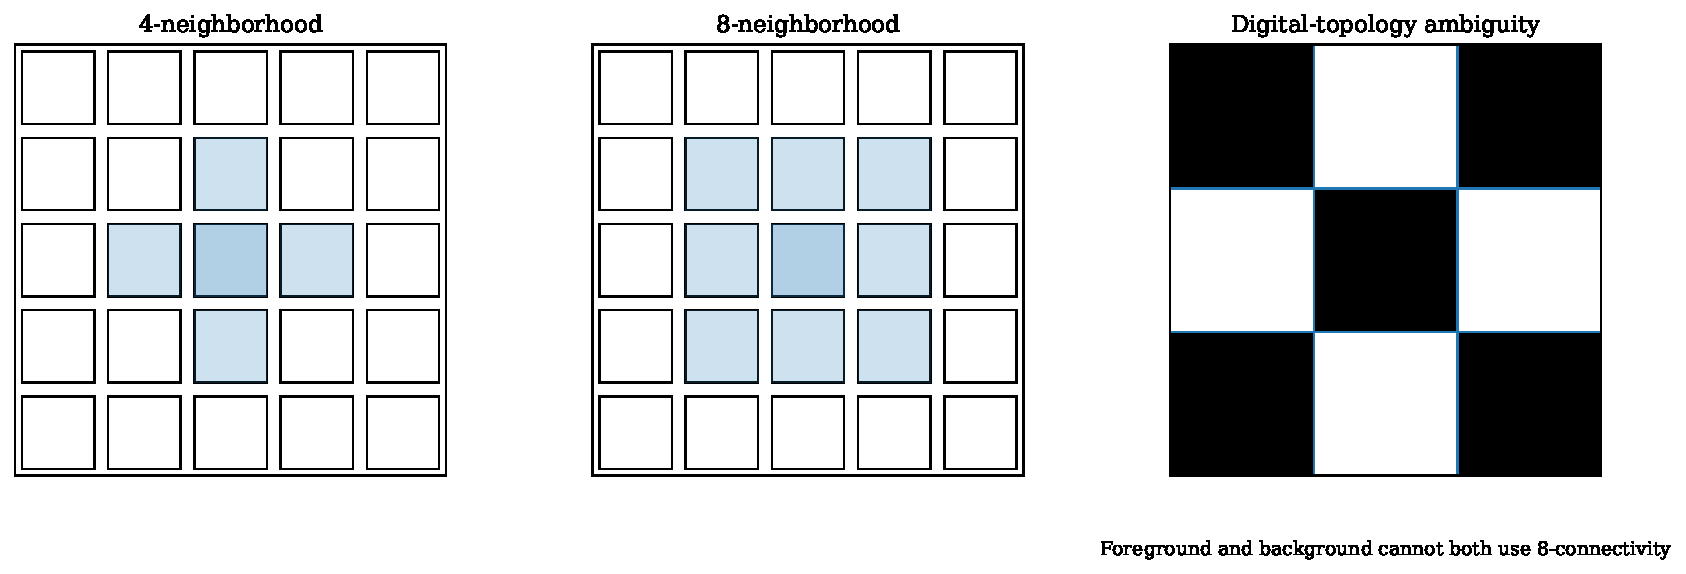
\includegraphics[width=.82\textwidth]{neighborhood_connectivity.pdf}
\caption{همسایگی‌های دیجیتال و اثر انتخاب اتصال بر مؤلفه‌های متصل.}
\end{figure}

\subsection{مؤلفه متصل و مشخصه اویلر}
رابطه هم‌ارزی «وجود مسیر دیجیتال» دامنه را به مؤلفه‌های متصل تقسیم می‌کند. در دوبعد، مشخصه اویلر
\begin{equation}
\chi=\beta_0-\beta_1
\end{equation}
است؛ \(\beta_0\) تعداد مؤلفه‌ها و \(\beta_1\) تعداد حفره‌هاست. این کمیت یک آزمون فشرده برای حفظ توپولوژی
در thinning، skeletonization و شبکه‌های قطعه‌بندی است.

\subsection{الگوریتم برچسب‌گذاری مؤلفه‌ها}
روش دوگذر کلاسیک در گذر اول برچسب موقت و روابط هم‌ارزی تولید و در گذر دوم هر برچسب را به نماینده مجموعه
اتحاد-یافت نگاشت می‌کند. پیچیدگی با فشرده‌سازی مسیر و اتحاد بر حسب رتبه عملاً خطی است:
\begin{equation}
T(N)=O(N\alpha(N))\approx O(N).
\end{equation}

\begin{algorithmbox}{الگوریتم ۷.۱: برچسب‌گذاری دوگذر}
\begin{enumerate}
\item تصویر را به ترتیب سطری پیمایش کنید؛ برای هر پیکسل پیش‌زمینه، برچسب همسایه‌های قبلاً دیده‌شده را بخوانید.
\item اگر هیچ برچسبی نیست، برچسب تازه بسازید؛ اگر یک یا چند برچسب هست، کمینه را اختصاص و برچسب‌ها را union کنید.
\item در گذر دوم، هر برچسب را با ریشه ساختار union--find جایگزین کنید.
\item ویژگی‌های جزء مانند مساحت، جعبه محاطی، مرکز جرم و محیط را در همان گذر تجمع دهید.
\end{enumerate}
\end{algorithmbox}

\section{ساختار دیفرانسیلی محلی و فضای مقیاس}
برای تصویر پیوسته \(f(x,y)\)، گرادیان
\begin{equation}
\nabla f=\begin{bmatrix}f_x&f_y\end{bmatrix}^{\!T}
\end{equation}
جهت بیشترین افزایش و قدر آن شدت تغییر را بیان می‌کند. مشتقات مرتبه دوم در هسین
\begin{equation}
H_f=\begin{bmatrix}f_{xx}&f_{xy}\\ f_{xy}&f_{yy}\end{bmatrix}
\end{equation}
خمیدگی محلی را در همه جهت‌ها رمز می‌کنند.

\subsection{چرا مشتق مستقیم نامناسب است؟}
مشتق، فرکانس بالا و در نتیجه نویز را تقویت می‌کند. راه اصولی، مشتق‌گیری از تصویر هموارشده است:
\begin{equation}
L(x,y;\sigma)=G_\sigma*f,\qquad
\partial_x L=(\partial_xG_\sigma)*f.
\end{equation}
فضای مقیاس گاوسی تنها خانواده خطی، ناوردا به انتقال و نیم‌گروهی است که ساختارهای جدید کاذب ایجاد نمی‌کند.

\begin{figure}[H]
\centering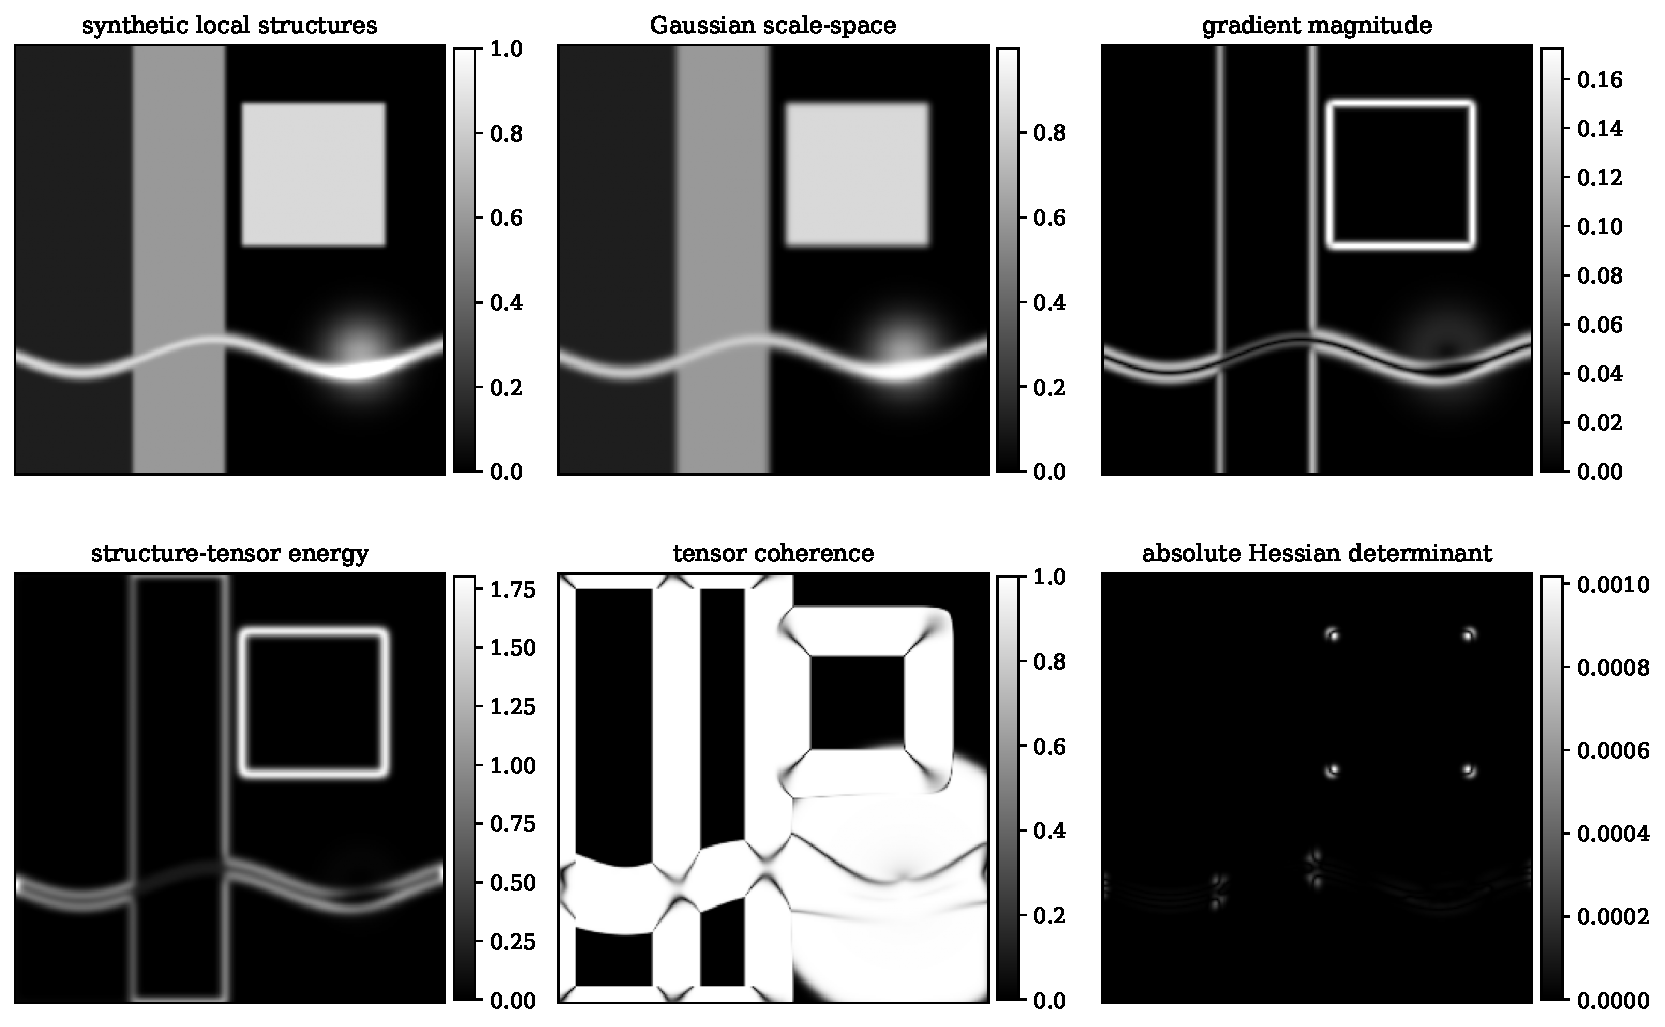
\includegraphics[width=.92\textwidth]{local_differential_structure.pdf}
\caption{ساختار دیفرانسیلی محلی در مقیاس‌های مختلف: گرادیان، پاسخ هسین و حساسیت به نویز.}
\end{figure}

\subsection{مشتق جهت‌دار و هموردایی چرخش}
برای بردار واحد \(u=(\cos\theta,\sin\theta)^T\)،
\begin{equation}
D_u f=u^T\nabla f.
\end{equation}
اگر تصویر بچرخد، گرادیان نیز با همان دوران می‌چرخد؛ بنابراین قدر گرادیان ناوردای چرخش و جهت آن همورداست.
این تمایز برای طراحی ویژگی صحیح حیاتی است.

\section{تانسور ساختار: از لبه تا گوشه}
تانسور ساختار در مقیاس مشتق \(\sigma\) و مقیاس تجمیع \(\rho\) تعریف می‌شود:
\begin{equation}
J_{\rho,\sigma}=G_\rho*\left(\nabla L_\sigma\nabla L_\sigma^T\right)
=\begin{bmatrix}
G_\rho*L_x^2&G_\rho*L_xL_y\\
G_\rho*L_xL_y&G_\rho*L_y^2
\end{bmatrix}.
\end{equation}
برای جابه‌جایی کوچک \(d\)، تغییر انرژی وصله تقریباً
\begin{equation}
E(d)\approx d^TJd
\end{equation}
است. اگر \(\lambda_1\ge\lambda_2\) مقادیر ویژه باشند، سه حالت رخ می‌دهد: هر دو کوچک ناحیه تخت؛ یکی بزرگ
لبه؛ و هر دو بزرگ گوشه یا ساختار دوبعدی.

\begin{figure}[H]
\centering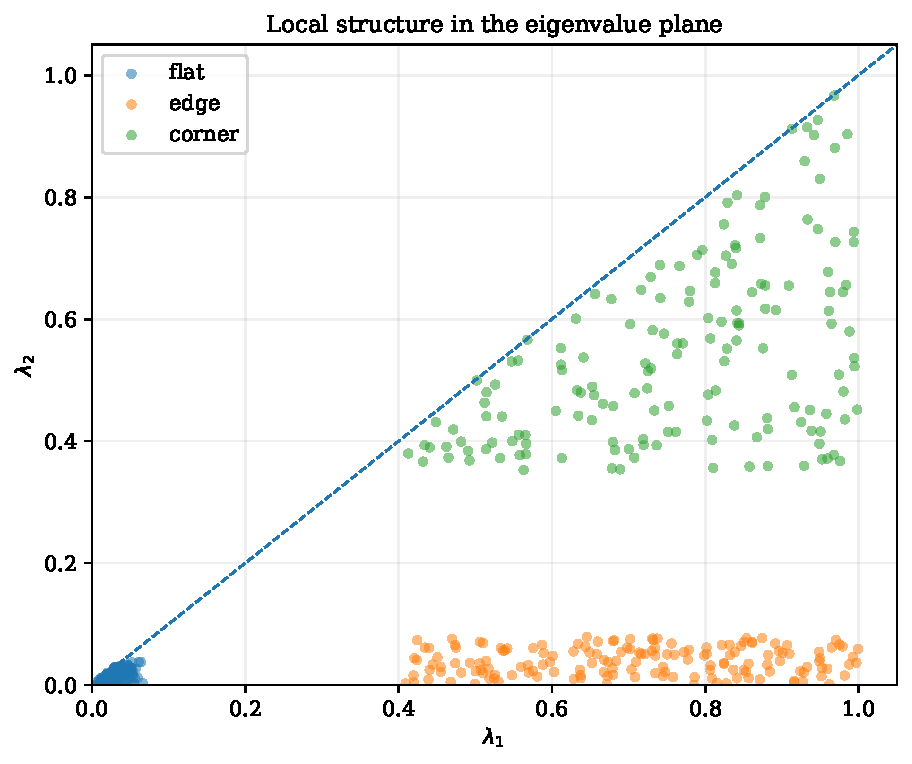
\includegraphics[width=.78\textwidth]{structure_tensor_eigenplane.pdf}
\caption{صفحه مقادیر ویژه تانسور ساختار و نواحی متناظر با تخت، لبه و گوشه.}
\end{figure}

\subsection{معیار هریس و شای-توماسی}
معیار هریس
\begin{equation}
R=\det J-k(\operatorname{tr}J)^2
\end{equation}
و معیار شای-توماسی \(R_{ST}=\min(\lambda_1,\lambda_2)\) است. هریس به مقیاس شدت حساس است؛ لذا نرمال‌سازی،
آستانه نسبی و non-maximum suppression باید بخشی از الگوریتم باشند، نه جزئیات حاشیه‌ای.

\begin{algorithmbox}{الگوریتم ۷.۲: آشکارساز گوشه مقیاس‌آگاه}
\begin{enumerate}
\item مشتقات گاوسی را در چند \(\sigma\) محاسبه کنید.
\item برای هر مقیاس، تانسور ساختار را با پنجره \(\rho\ge\sigma\) بسازید.
\item پاسخ گوشه را با توان مناسب مقیاس نرمال کنید.
\item بیشینه‌های موضعی فضایی-مقیاسی را استخراج و نقاط نزدیک مرز یا با شرطی‌بودن نامناسب را حذف کنید.
\item کوواریانس مکان نقطه را از وارون هسین پاسخ تخمین بزنید.
\end{enumerate}
\end{algorithmbox}

\section{هسین، خط و ساختارهای لوله‌ای}
مقادیر ویژه هسین تفاوت خمیدگی در دو جهت اصلی را نشان می‌دهند. در یک ridge روشن باریک، یکی از مقادیر ویژه
منفی با قدر بزرگ و دیگری نزدیک صفر است. پاسخ چندمقیاسی vesselness را می‌توان به صورت
\begin{equation}
V_\sigma=\exp\!\left(-\frac{R_B^2}{2\beta^2}\right)
\left[1-\exp\!\left(-\frac{S^2}{2c^2}\right)\right],
\quad R_B=\frac{|\lambda_1|}{|\lambda_2|},\quad S=\sqrt{\lambda_1^2+\lambda_2^2}
\end{equation}
نوشت. انتخاب بیشینه روی مقیاس، قطر تقریبی ساختار را نیز تخمین می‌زند.

\section{از فیلتر جهت‌دار تا کدهای محلی}
فیلترهای steerable اجازه می‌دهند پاسخ هر زاویه از ترکیب خطی تعداد محدودی فیلتر پایه ساخته شود. برای مشتق
گاوسی مرتبه اول،
\begin{equation}
G_\theta^{(1)}=\cos\theta\,G_x+\sin\theta\,G_y.
\end{equation}
در مقابل، الگوی دودویی محلی با مقایسه شدت همسایه و مرکز
\begin{equation}
\operatorname{LBP}_{P,R}=\sum_{p=0}^{P-1}\mathbf 1[g_p\ge g_c]2^p
\end{equation}
یک کد ترتیبی مقاوم به تبدیل‌های یکنوای شدت می‌سازد. این دو خانواده نشان می‌دهند که «محلی» می‌تواند هم
تحلیلی-پیوسته و هم ترتیبی-گسسته باشد.

\section{مبانی جبری مورفولوژی ریاضی}
\subsection{مشبکه کامل}
مجموعه تصاویر خاکستری با ترتیب نقطه‌ای \(f\le g\iff f(x)\le g(x)\) یک مشبکه کامل است؛ سوپریمم و اینفیمم
به صورت نقطه‌ای محاسبه می‌شوند. dilation عملگری است که سوپریمم‌ها را حفظ می‌کند و erosion اینفیمم‌ها را.

\subsection{اتصال گالوا و adjunction}
زوج \((\varepsilon,\delta)\) یک adjunction است اگر
\begin{equation}
\delta(f)\le g\quad\Longleftrightarrow\quad f\le\varepsilon(g).
\end{equation}
از همین رابطه افزایش‌پذیری، تعریف opening \(\gamma=\delta\varepsilon\) و closing
\(\varphi=\varepsilon\delta\)، و خواص ضدگسترده/گسترده و idempotent استخراج می‌شوند.

\begin{theorembox}{قضیه: opening و closing}
اگر \((\varepsilon,\delta)\) یک adjunction باشد، \(\gamma=\delta\varepsilon\) افزایشی، ضدگسترده و idempotent
است؛ \(\varphi=\varepsilon\delta\) افزایشی، گسترده و idempotent است.
\end{theorembox}

\subsection{اثبات فشرده}
از adjunction با \(g=\varepsilon(f)\) داریم \(\delta\varepsilon(f)\le f\). افزایش‌پذیری از افزایش‌پذیری اعضا
می‌آید. با اعمال \(\gamma\) بر نامساوی ضدگستردگی و استفاده از افزایش‌پذیری،
\(\gamma\gamma(f)\le\gamma(f)\)؛ و چون \(\gamma(f)\le f\)، از افزایش‌پذیری و تعریف adjunction جهت عکس حاصل
می‌شود. استدلال closing دوگان است.

\section{مورفولوژی دودویی}
برای \(X,B\subseteq E\)، dilation و erosion به ترتیب
\begin{align}
X\oplus B&=\{x:\check B_x\cap X\neq\varnothing\},\\
X\ominus B&=\{x:B_x\subseteq X\}.
\end{align}
تعریف‌های جمع مینکوفسکی متناظر عبارت‌اند از
\begin{equation}
X\oplus B=\{x+b:x\in X,b\in B\},\qquad
X\ominus B=\{x:x+B\subseteq X\}.
\end{equation}

\begin{figure}[H]
\centering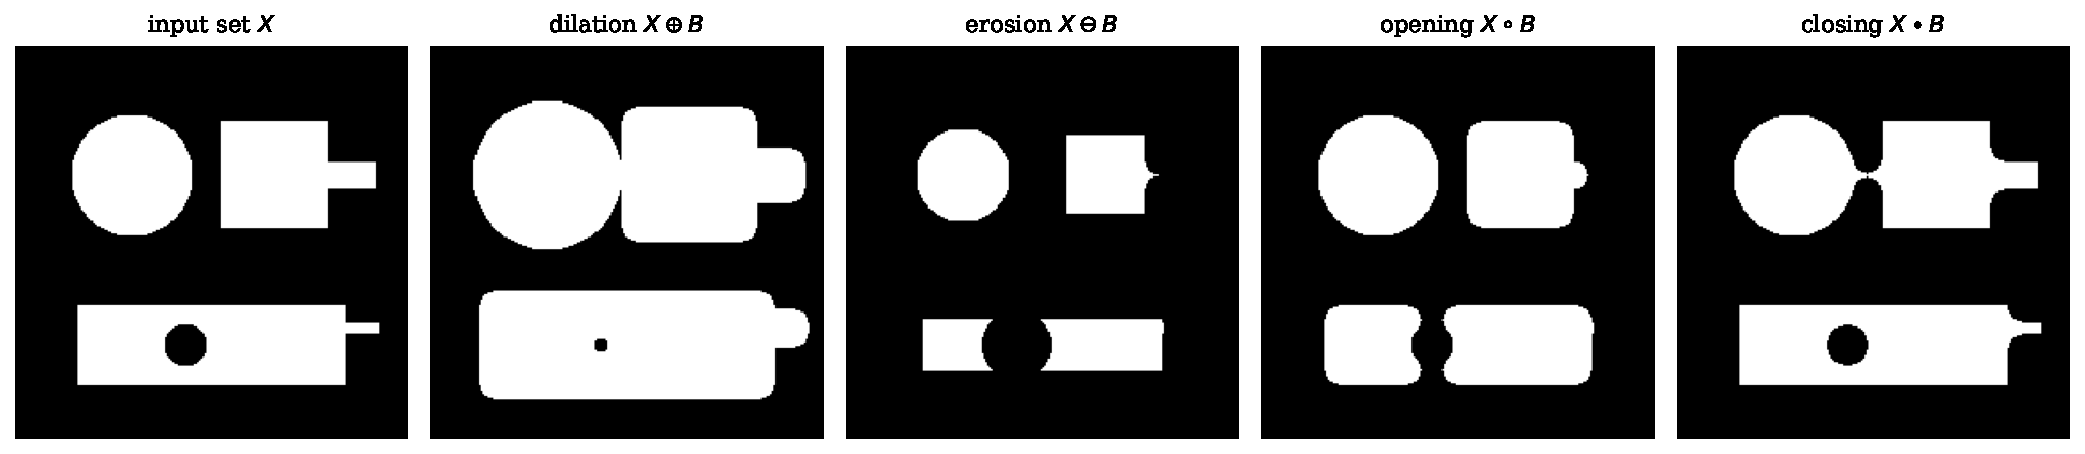
\includegraphics[width=.92\textwidth]{binary_morphology.pdf}
\caption{اثر dilation، erosion، opening و closing دودویی با عناصر ساختاری مختلف.}
\end{figure}

\subsection{تبدیل hit-or-miss}
برای عنصر مرکب \(B=(B_1,B_0)\) با قیود پیش‌زمینه و پس‌زمینه،
\begin{equation}
X\circledast B=(X\ominus B_1)\cap(X^c\ominus B_0)
\end{equation}
الگوی دقیق محلی را آشکار می‌کند و پایه thinning، thickening و تشخیص نقاط انتهایی است.

\subsection{انتخاب عنصر ساختاری}
عنصر ساختاری یک prior هندسی صریح است. دیسک برای ناوردایی تقریبی چرخش، خط برای ساختار جهت‌دار، مستطیل
برای شبکه‌های محورهم‌راستا و footprint داده‌محور برای کاربرد تخصصی مناسب است. اندازه باید در واحد فیزیکی
گزارش شود؛ یک شعاع ۵ پیکسلی در دو رزولوشن، یک معنای هندسی ندارد.

\section{مورفولوژی خاکستری و هندسه max-plus}
برای عنصر ساختاری غیرتخت \(b\bar{:}B\to\mathbb R\)،
\begin{align}
(\delta_b f)(x)&=\sup_{y\in B}\{f(x-y)+b(y)\},\\
(\varepsilon_b f)(x)&=\inf_{y\in B}\{f(x+y)-b(y)\}.
\end{align}
این روابط کانولوشن max-plus و min-plus هستند. مورفولوژی خاکستری بنابراین «کانولوشن غیرخطی روی نیم‌حلقه
idempotent» است، نه نسخه‌ای تجربی از max-pooling.

\begin{figure}[H]
\centering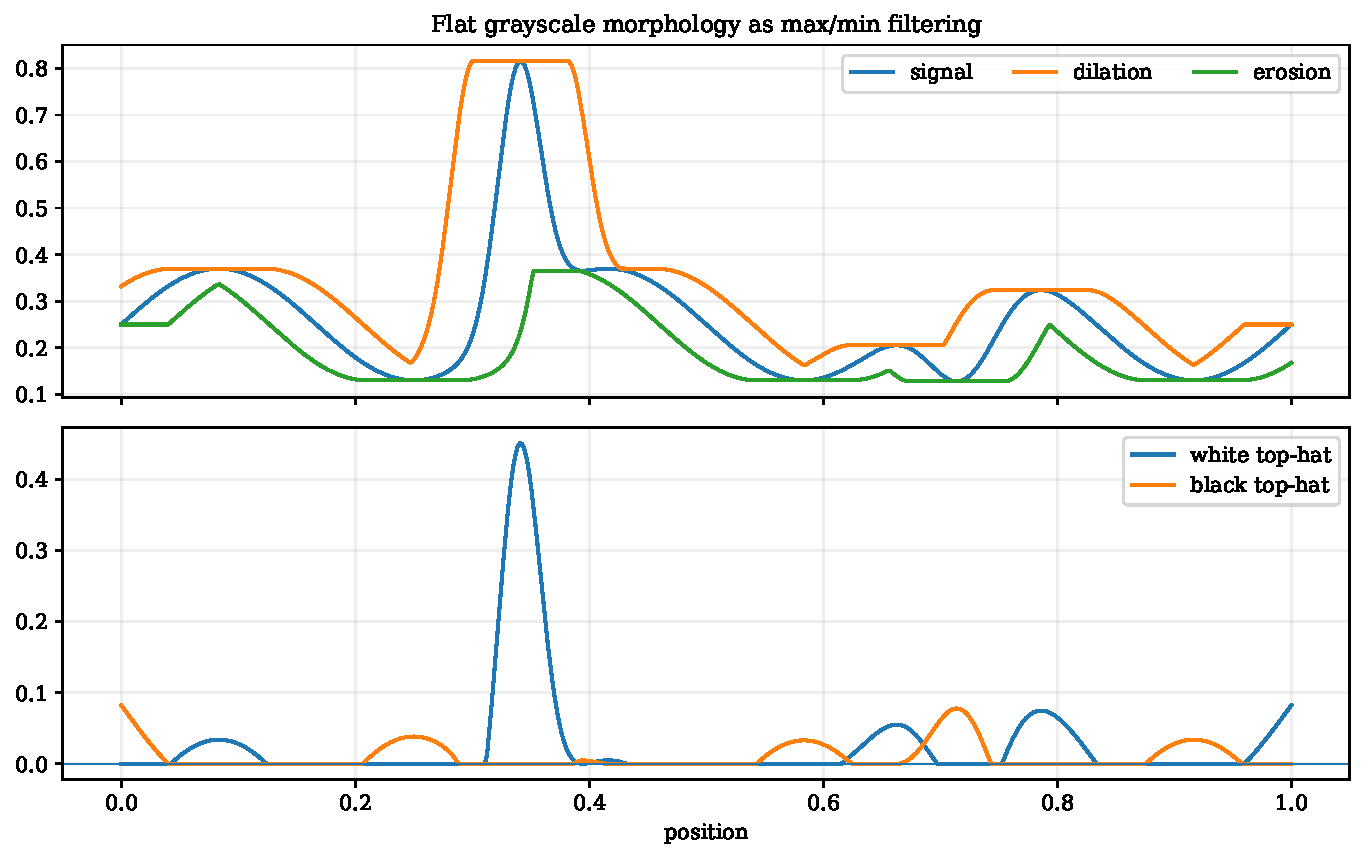
\includegraphics[width=.9\textwidth]{grayscale_morphology_profiles.pdf}
\caption{پروفایل یک‌بعدی dilation و erosion تخت و غیرتخت و اثر آن‌ها بر قله و دره.}
\end{figure}

\subsection{گرادیان و top-hat مورفولوژیک}
\begin{align}
\nabla_B f&=\delta_Bf-\varepsilon_Bf,\\
T_w(f)&=f-\gamma_B(f),\\
T_b(f)&=\varphi_B(f)-f.
\end{align}
گرادیان مرز را برجسته می‌کند؛ white top-hat ساختارهای روشن کوچک‌تر از \(B\) و black top-hat ساختارهای
تیره را استخراج می‌کند.

\section{الگوریتم‌های سریع dilation و erosion}
محاسبه ساده پنجره با اندازه \(k\) روی \(N\) پیکسل، \(O(Nk)\) است. برای عنصر خطی تخت، الگوریتم van Herk/Gil-Werman
در هر بعد با تعداد مقایسه ثابت مستقل از \(k\) کار می‌کند.

\begin{algorithmbox}{الگوریتم ۷.۳: بیشینه لغزان van Herk در یک بعد}
\begin{enumerate}
\item سیگنال را به بلوک‌های طول \(k\) تقسیم کنید.
\item آرایه پیشوند \(g[i]\) را با بیشینه از ابتدای هر بلوک تا \(i\) بسازید.
\item آرایه پسوند \(h[i]\) را با بیشینه از انتهای هر بلوک تا \(i\) بسازید.
\item بیشینه پنجره مرکز \(i\) را از بیشینه دو مقدار مناسب \(h[i-r]\) و \(g[i+r]\) به دست آورید.
\item برای مستطیل دوبعدی، الگوریتم را separable روی سطر و ستون اجرا کنید.
\end{enumerate}
پیچیدگی \(O(N)\)، حافظه \(O(N)\) یا در نسخه جریانی \(O(k)\) است.
\end{algorithmbox}

\section{بازسازی مورفولوژیک و عملگرهای ژئودزیک}
در بازسازی با marker \(g\le f\) و mask \(f\)، dilation ژئودزیک
\begin{equation}
\delta_f^{(1)}(g)=\min(\delta_Bg,f)
\end{equation}
تکرار می‌شود تا نقطه ثابت
\begin{equation}
R_f^\delta(g)=\delta_f^{(\infty)}(g)
\end{equation}
حاصل شود. برخلاف opening معمولی، بازسازی اجزای مجاز را بدون تغییر شکل اصلی بازیابی می‌کند.

\begin{figure}[H]
\centering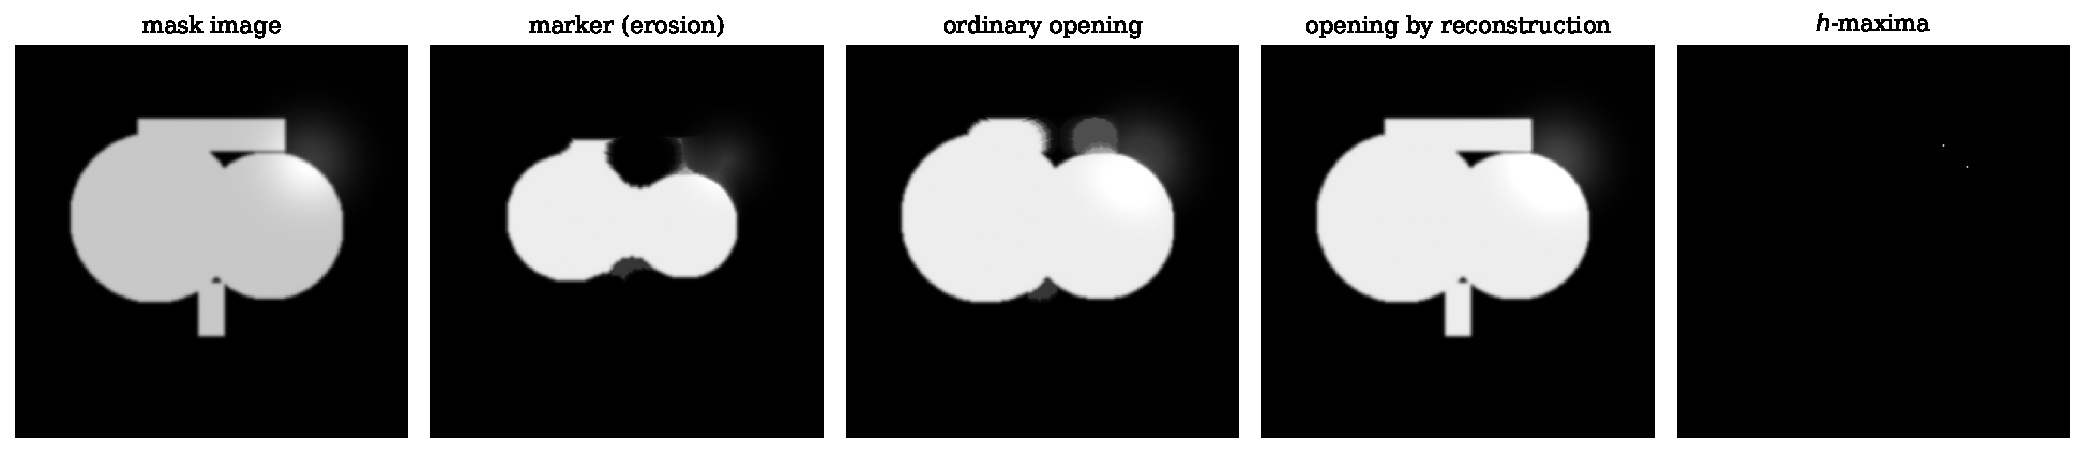
\includegraphics[width=.9\textwidth]{morphological_reconstruction.pdf}
\caption{بازسازی مورفولوژیک از marker زیر mask و تفاوت آن با opening معمولی.}
\end{figure}

\begin{algorithmbox}{الگوریتم ۷.۴: بازسازی سریع صف‌محور}
\begin{enumerate}
\item یک پیمایش رو به جلو و یک پیمایش رو به عقب برای انتشار اولیه مقادیر انجام دهید.
\item پیکسل‌هایی را که هنوز می‌توانند همسایه‌ای را افزایش دهند وارد صف FIFO کنید.
\item تا خالی شدن صف، مقدار همسایه \(q\) را با \(\min(f(q),g(p))\) به‌روزرسانی کنید.
\item اگر مقدار \(q\) افزایش یافت، آن را وارد صف کنید.
\end{enumerate}
هر افزایش محدود است و الگوریتم در عمل نزدیک \(O(N)\) است.
\end{algorithmbox}

\subsection{h-maxima و حذف قله‌های کم‌اهمیت}
\begin{equation}
H_h(f)=f-R_f^\delta(f-h)
\end{equation}
قله‌هایی با برجستگی کمتر از \(h\) را حذف می‌کند. این عملگر برای تولید markerهای پایدار watershed از threshold
ساده مناسب‌تر است.

\section{عملگرهای متصل و درخت‌های مؤلفه}
عملگر متصل مرز اجزای باقی‌مانده را جابه‌جا نمی‌کند؛ فقط اجزا را نگه می‌دارد یا حذف/ادغام می‌کند. max-tree
مؤلفه‌های متصل مجموعه‌های تراز بالا
\begin{equation}
X_\lambda=\{x:f(x)\ge\lambda\}
\end{equation}
را در یک سلسله‌مراتب inclusion سازمان می‌دهد. هر گره یک جزء و هر یال رابطه والد در سطح پایین‌تر است.

\begin{figure}[H]
\centering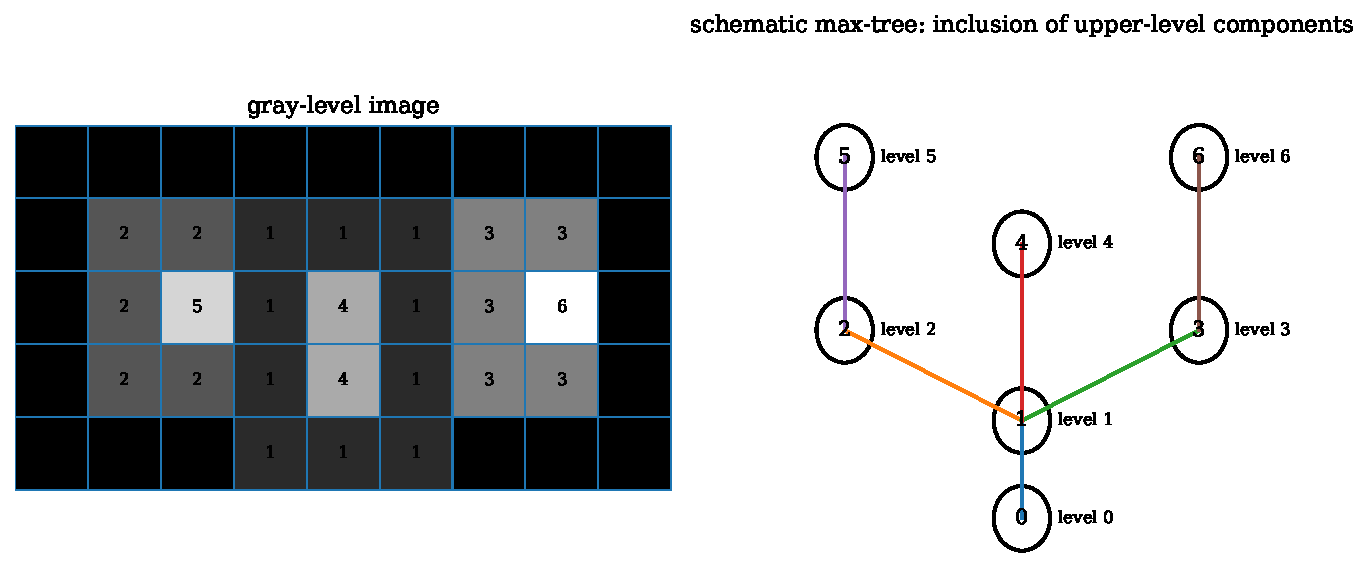
\includegraphics[width=.88\textwidth]{component_tree_schematic.pdf}
\caption{نمای شماتیک max-tree و نگاشت نواحی سطح بالا به گره‌های سلسله‌مراتبی.}
\end{figure}

\subsection{فیلترهای ویژگی}
اگر ویژگی گره \(A(C)\) مانند مساحت، ارتفاع، واریانس یا elongation باشد، pruning درخت بر اساس شرط
\(A(C)\ge\tau\) یک فیلتر متصل می‌سازد. ویژگی باید افزایش‌پذیر باشد تا threshold ساده سازگاری سلسله‌مراتبی
داشته باشد؛ در غیر این صورت قواعد pruning پیچیده‌تری لازم است.

\begin{algorithmbox}{الگوریتم ۷.۵: ساخت max-tree با union--find}
\begin{enumerate}
\item پیکسل‌ها را به ترتیب نزولی شدت مرتب یا با histogram bucket کنید.
\item پیکسل‌ها را سطح‌به‌سطح فعال کنید و برای هر پیکسل، مجموعه همسایه‌های فعال را union کنید.
\item هنگام ادغام اجزای سطوح متفاوت، گره والد-فرزند ثبت کنید.
\item پس از canonicalization، ویژگی‌ها را از برگ به ریشه تجمع دهید.
\end{enumerate}
پیچیدگی عمومی \(O(N\log N)\) به علت مرتب‌سازی و برای دامنه شدت محدود نزدیک \(O(N\alpha(N))\) است.
\end{algorithmbox}

\section{تبدیل فاصله و min-convolution}
برای مجموعه پیش‌زمینه \(X\)، تبدیل فاصله اقلیدسی
\begin{equation}
D_X(p)=\min_{q\in X^c}\|p-q\|_2
\end{equation}
است. نسخه مربع فاصله یک تابع دوبعدی separable است و به دو تبدیل یک‌بعدی
\begin{equation}
D(i)=\min_j\{f(j)+(i-j)^2\}
\end{equation}
تقلیل می‌یابد؛ یعنی پوش پایین سهمی‌ها.

\begin{figure}[H]
\centering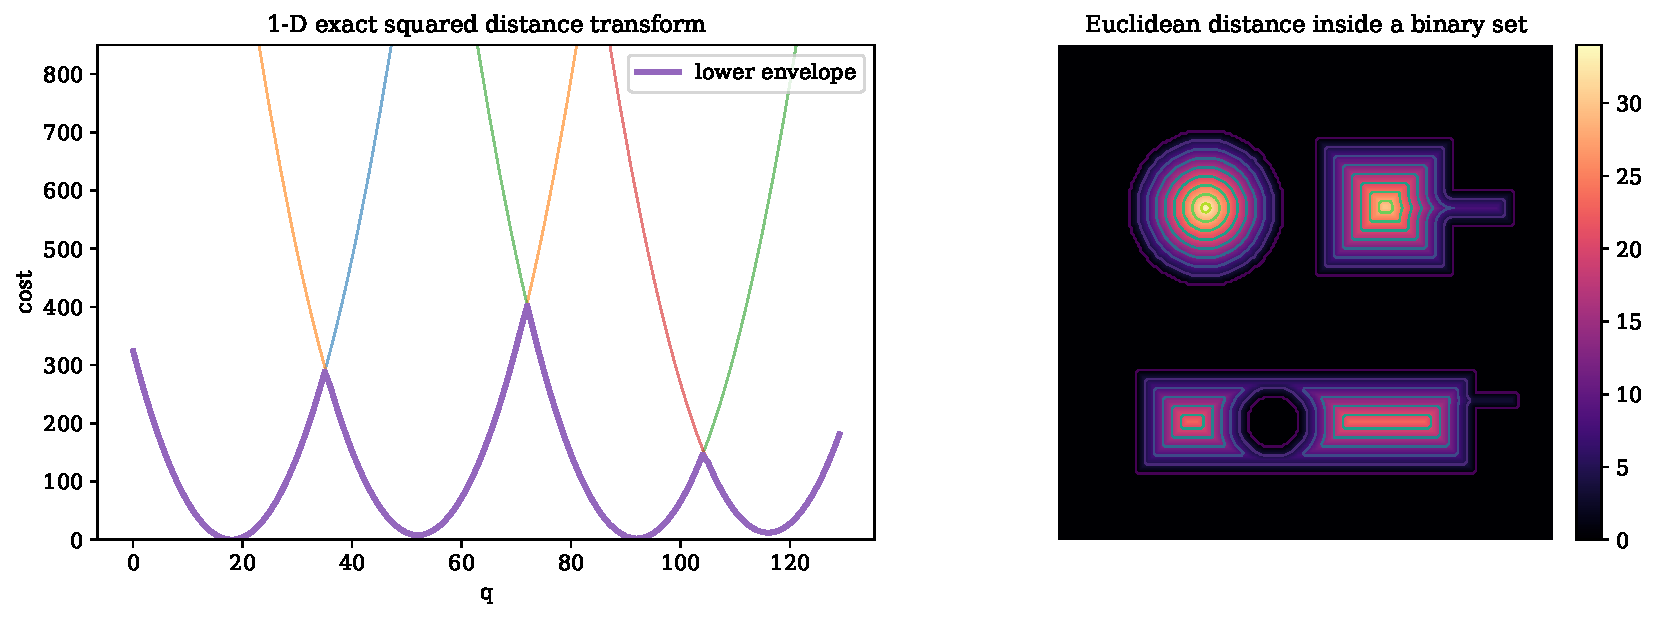
\includegraphics[width=.9\textwidth]{distance_transform_parabolas.pdf}
\caption{تبدیل فاصله دقیق به‌صورت پوش پایین سهمی‌ها؛ اساس الگوریتم خطی فلزن‌سوالب--هاتن‌لوخر.}
\end{figure}

\begin{algorithmbox}{الگوریتم ۷.۶: EDT دقیق خطی در یک بعد}
\begin{enumerate}
\item آرایه \(v\) اندیس سهمی‌های فعال و \(z\) محل تقاطع متوالی آن‌ها را نگه می‌دارد.
\item برای هر سهمی جدید، محل تقاطع با سهمی آخر را محاسبه کنید؛ تا وقتی تقاطع چپ‌تر از مرز قبلی است، سهمی آخر را حذف کنید.
\item سهمی جدید و مرز اعتبار آن را اضافه کنید.
\item در گذر دوم، برای هر \(i\) سهمی فعال متناظر با بازه \(z\) را ارزیابی کنید.
\end{enumerate}
هر سهمی حداکثر یک بار وارد و یک بار حذف می‌شود؛ پس زمان \(O(n)\) است.
\end{algorithmbox}

\section{محور میانی، اسکلت و thinning}
محور میانی مکان مراکز توپ‌های بیشینه محاط در شکل است. اگر \(D_X\) تبدیل فاصله باشد، ridgeهای آن تقریب محور
میانی‌اند. اسکلت همراه با شعاع، امکان بازسازی شکل را فراهم می‌کند:
\begin{equation}
X=\bigcup_{p\in\operatorname{MA}(X)}B(p,D_X(p)).
\end{equation}

\begin{figure}[H]
\centering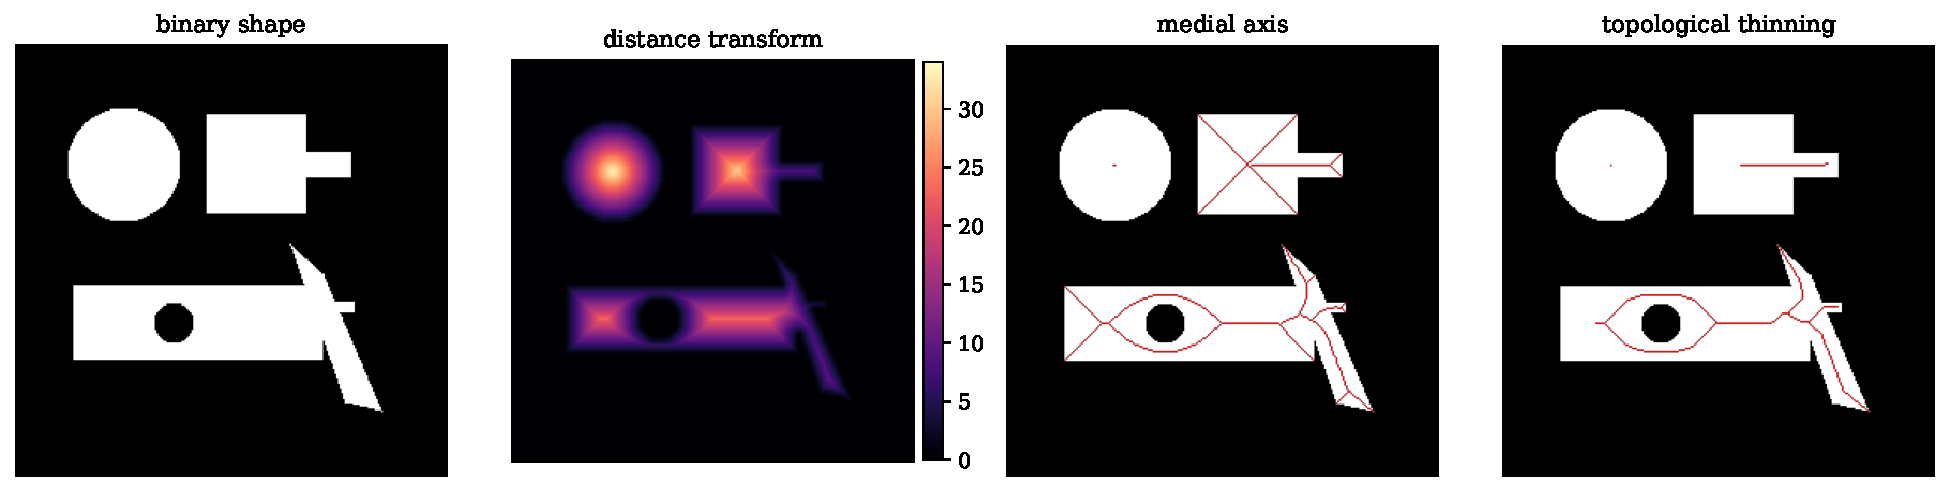
\includegraphics[width=.9\textwidth]{skeleton_medial_axis.pdf}
\caption{تفاوت محور میانی هندسی، skeleton یک‌پیکسلی و اثر شاخه‌های کاذب ناشی از ناهمواری مرز.}
\end{figure}

\subsection{نقطه ساده و حفظ توپولوژی}
پیکسل \(p\) ساده است اگر حذف آن تعداد مؤلفه‌های پیش‌زمینه و پس‌زمینه را تغییر ندهد. thinning توپولوژیک
پیکسل‌های مرزی ساده را با قیود endpoint و جهت به‌طور تکراری حذف می‌کند.

\begin{algorithmbox}{الگوریتم ۷.۷: thinning زیرچرخه‌ای}
\begin{enumerate}
\item پیکسل‌های مرزی را در یک یا چند جهت کاندید کنید.
\item برای هر کاندید، تعداد انتقال صفر به یک در حلقه ۸-همسایگی و تعداد همسایه‌های پیش‌زمینه را محاسبه کنید.
\item تنها نقاط ساده‌ای را حذف کنید که endpoint نیستند و قیود جهت زیرچرخه را برآورده می‌کنند.
\item زیرچرخه‌های مکمل را تا نبود تغییر تکرار کنید.
\end{enumerate}
حذف هم‌زمان بدون زیرچرخه می‌تواند اتصال را بشکند؛ بنابراین ترتیب بخشی از اثبات الگوریتم است.
\end{algorithmbox}

\subsection{هرس اسکلت}
شاخه‌های کوتاه معمولاً حاصل نویز مرز هستند. هرس باید بر اساس طول ژئودزیک، persistence، نسبت طول به شعاع یا
اهمیت بازسازی انجام شود؛ حذف صرفاً بر حسب تعداد پیکسل به رزولوشن وابسته است.

\section{watershed: از توپوگرافی تا جنگل پوشای کمینه}
تصویر گرادیان را سطح ارتفاع در نظر بگیرید. watershed مرز حوضه‌های آبریز مینیمم‌ها را می‌سازد. نسخه naive
به‌علت تعداد زیاد مینیمم‌های نویزی over-segmentation شدید دارد؛ راه حل عملی، marker-controlled watershed است.

\begin{figure}[H]
\centering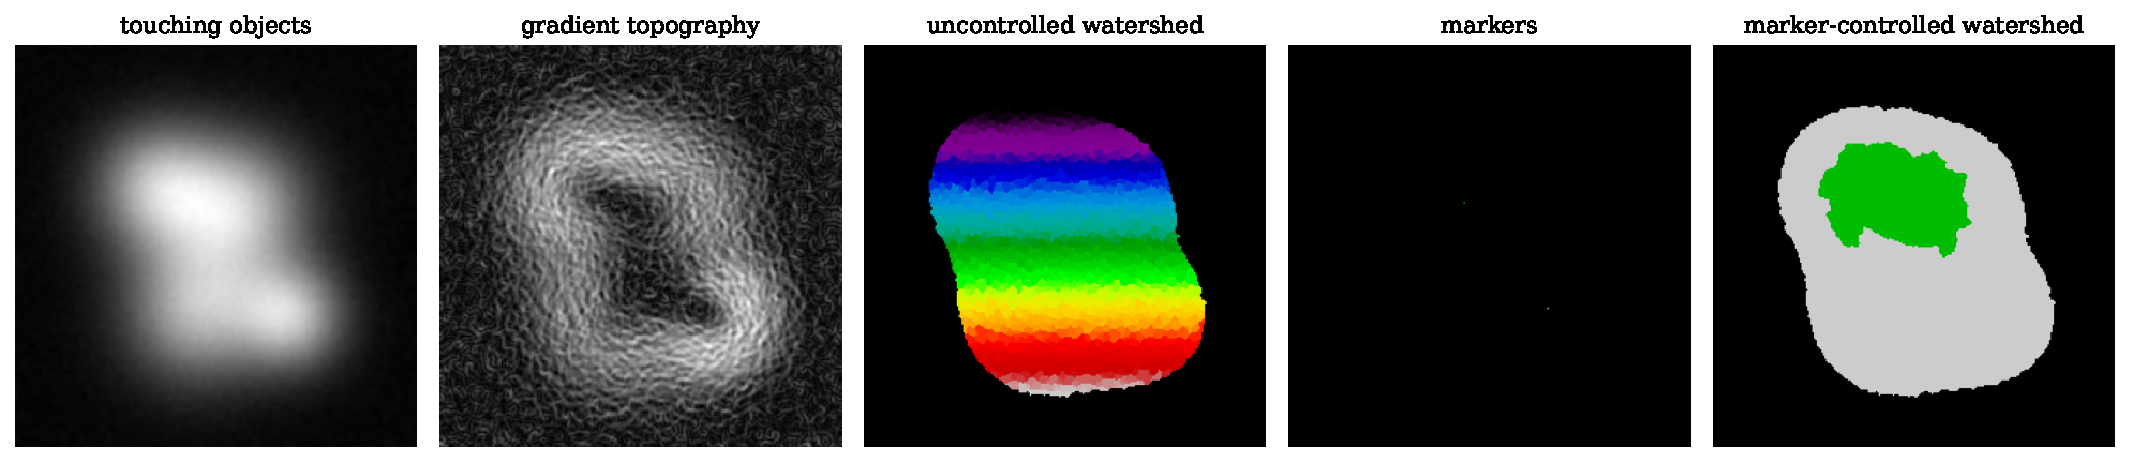
\includegraphics[width=.94\textwidth]{watershed_marker_controlled.pdf}
\caption{watershed نشان‌محور: تولید marker، سطح گرادیان و جداسازی اشیای چسبیده.}
\end{figure}

\subsection{صورت‌بندی گرافی}
روی گراف پیکسل‌ها با وزن یال
\begin{equation}
w(p,q)=\max(g(p),g(q))
\end{equation}
یا اختلاف شدت، watershed نشان‌دار با جنگل پوشای کمینه ریشه‌دار مرتبط است. هر رأس به markerی متصل می‌شود که
هزینه مسیر minimax آن کمینه است.

\begin{algorithmbox}{الگوریتم ۷.۸: watershed با صف اولویت}
\begin{enumerate}
\item markerها را با برچسب‌های متمایز مقداردهی و همسایه‌های بدون برچسب آن‌ها را در صف اولویت بر حسب ارتفاع وارد کنید.
\item کم‌ارتفاع‌ترین پیکسل را خارج کنید.
\item اگر همسایه‌های برچسب‌دار آن یک برچسب واحد دارند، همان را اختصاص دهید؛ اگر چند برچسب دارند، مرز watershed ثبت کنید.
\item همسایه‌های تازه را وارد صف کنید تا صف خالی شود.
\end{enumerate}
با heap زمان \(O(N\log N)\) و با bucket queue برای شدت محدود نزدیک \(O(N)\) است.
\end{algorithmbox}

\section{گرانولومتری و طیف الگو}
خانواده openingهای \(\gamma_r\) با عناصر ساختاری افزاینده یک sieve مورفولوژیک می‌سازد. اگر \(V(f)\) حجم
تصویر باشد، تابع اندازه
\begin{equation}
G(r)=1-\frac{V(\gamma_r(f))}{V(f)}
\end{equation}
و مشتق گسسته آن pattern spectrum توزیع اندازه ساختارها را تقریب می‌زند.

\begin{figure}[H]
\centering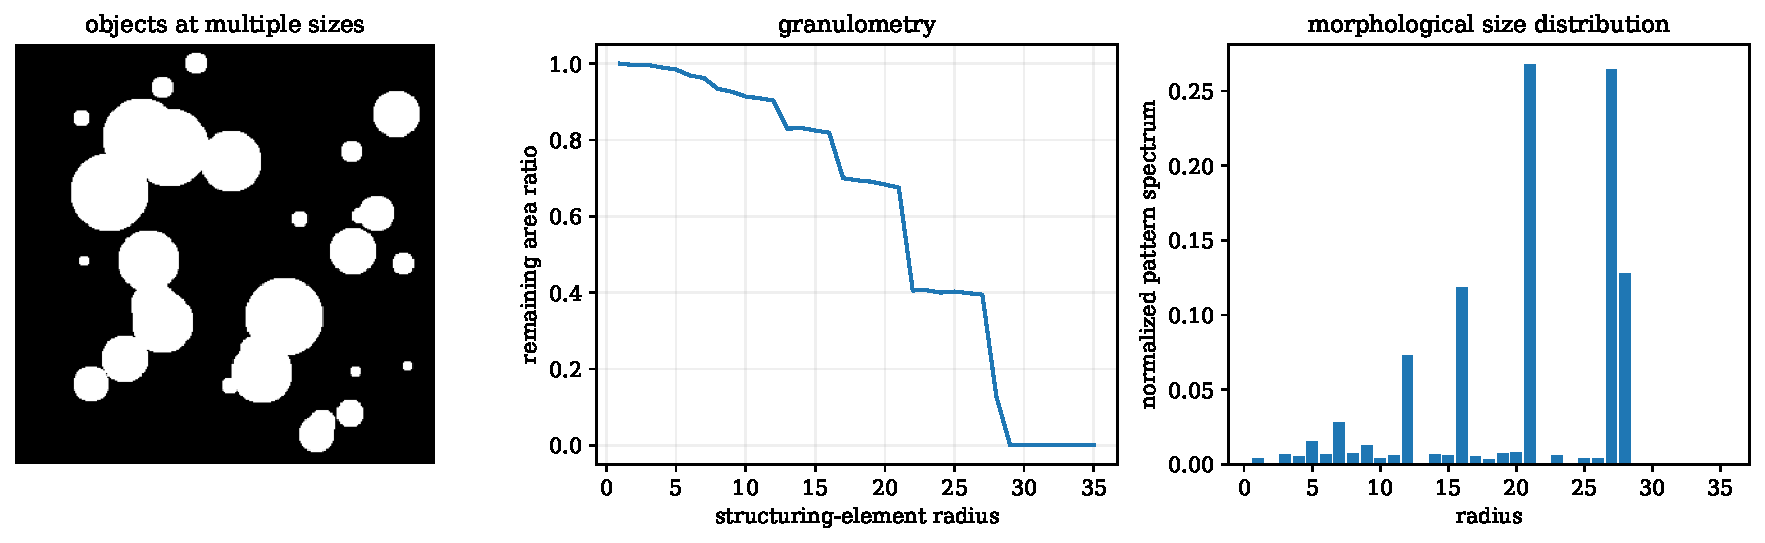
\includegraphics[width=.9\textwidth]{granulometry_pattern_spectrum.pdf}
\caption{گرانولومتری چندمقیاسی و طیف الگو برای مخلوطی از اجسام با اندازه‌های متفاوت.}
\end{figure}

\subsection{پروفایل مورفولوژیک}
بردار پاسخ opening/closing در چند مقیاس
\begin{equation}
\operatorname{MP}(x)=\big[\gamma_{r_m}f(x),\ldots,\gamma_{r_1}f(x),f(x),
\varphi_{r_1}f(x),\ldots,\varphi_{r_m}f(x)\big]
\end{equation}
یک توصیف‌گر ساختاری برای سنجش‌ازدور، بافت و قطعه‌بندی است. differential morphological profile اختلاف بین
مقیاس‌های متوالی را استفاده می‌کند.

\section{اندازه‌گیری شکل و ناوردایی‌ها}
برای جزء \(X\)، مساحت \(A=|X|\)، مرکز جرم \(\mu\) و ماتریس ممان مرتبه دوم
\begin{equation}
C=\frac{1}{A}\sum_{x\in X}(x-\mu)(x-\mu)^T
\end{equation}
هستند. مقادیر ویژه \(C\) جهت اصلی و elongation را می‌دهند. compactness معمولاً
\begin{equation}
Q=\frac{4\pi A}{P^2}\le 1
\end{equation}
است، ولی محیط دیجیتال به جهت و روش برآورد حساس است. گزارش شکل بدون ذکر estimator محیط قابل تکرار نیست.

\subsection{ممان‌های ناوردا}
ممان‌های مرکزی نرمال‌شده نسبت به انتقال و مقیاس ناوردا هستند؛ ترکیب‌های Hu ناوردایی چرخش می‌سازند. در حضور
نویز مرز، ممان‌های مرتبه بالا ناپایدارند؛ لذا regularization مرز یا توصیف‌گرهای مبتنی بر distance transform
اغلب مناسب‌ترند.


\section{مورفولوژی برداری، رنگی و چندطیفی}
در تصویر چندکاناله، ترتیب طبیعی کامل وجود ندارد. اگر min و max مستقل کانالی اعمال شوند، ممکن است برداری تولید شود
که اصلاً در داده وجود نداشته و رنگ کاذب بسازد. بنابراین باید یک preorder یا نگاشت مرتب‌ساز
\(\rho:\mathbb R^d\to\mathbb R^m\) تعریف شود. سه راهبرد رایج عبارت‌اند از ترتیب حاشیه‌ای، ترتیب کاهش‌یافته
بر اساس یک scalarization، و ترتیب واژگانی.

برای ترتیب کاهش‌یافته با امتیاز \(s(v)\)، dilation برداری
\begin{equation}
(\delta_B f)(x)=f(x-y^*),\qquad
y^*=\arg\max_{y\in B}s(f(x-y))
\end{equation}
یکی از بردارهای واقعی پنجره را انتخاب می‌کند. انتخاب \(s\) باید با کاربرد سازگار باشد: روشنایی، فاصله ماهالانوبیس
از پس‌زمینه، عمق طیفی یا projection آموخته‌شده.

\begin{warningbox}
مورفولوژی مستقل روی کانال‌های RGB عموماً با هندسه رنگ سازگار نیست. برای تصویر رنگی، فضای رنگ، metric و
ترتیب بردار بخشی از تعریف عملگرند و باید همراه نتیجه گزارش شوند.
\end{warningbox}

\subsection{مورفولوژی ماتریسی و تانسوری}
برای داده‌های SPD مانند تانسور انتشار یا ماتریس کوواریانس، ترتیب Loewner جزئی است:
\begin{equation}
A\preceq B\iff B-A\succeq0.
\end{equation}
چون هر دو ماتریس الزاماً قابل مقایسه نیستند، sup/inf ممکن است یکتا نباشد. راه‌حل‌ها شامل embedding به فضای
اقلیدسی، میانگین‌های ریمانی و تعریف dilation بر حسب بهینه‌سازی انرژی است. این نمونه نشان می‌دهد انتقال
مورفولوژی از اسکالر به داده ساخت‌یافته یک مسئله جبری واقعی است.

\section{مورفولوژی روی گراف، مش و ابرنقاط}
شبکه پیکسلی تنها یک گراف خاص است. روی گراف \(G=(V,E)\)، همسایگی \(N(v)\) جای footprint انتقال‌پذیر را می‌گیرد:
\begin{align}
(\delta f)(v)&=\max_{u\in N[v]} f(u),\\
(\varepsilon f)(v)&=\min_{u\in N[v]} f(u).
\end{align}
اگر یال‌ها وزن‌دار باشند، عنصر ساختاری می‌تواند توپ متریک گراف
\(B_r(v)=\{u:d_G(u,v)\le r\}\) باشد. این تعریف برای superpixel graph، mesh، شبکه راه، مولکول و ابرنقطه مناسب است.

\subsection{فاصله ژئودزیک و propagation}
برای هزینه رأس \(c(v)\ge0\)، فاصله ژئودزیک وزنی
\begin{equation}
d_c(s,v)=\min_{\pi:s\leadsto v}\sum_{u\in\pi}c(u)
\end{equation}
است. رشد marker در این metric، نسخه‌ای از morphology ژئودزیک و پایه watershed، random walker و روش‌های
front propagation است. با هزینه نامنفی، Dijkstra زمان \(O(|E|\log|V|)\) دارد؛ روی bucketهای صحیح، Dial
می‌تواند سریع‌تر باشد.

\begin{algorithmbox}{الگوریتم ۷.۹: dilation گرافی با شعاع ژئودزیک}
\begin{enumerate}
\item از همه رأس‌های marker یک Dijkstra چندمبدأ آغاز کنید.
\item رأس‌ها را تا فاصله \(r\) گسترش دهید و مبدأ برنده را ثبت کنید.
\item در تساوی هزینه، قرارداد tie-breaking ثابت یا برچسب مرزی به کار ببرید.
\item برای erosion، dilation مکمل یا شرط قرارگیری کامل توپ متریک را استفاده کنید.
\end{enumerate}
\end{algorithmbox}

\subsection{ابرنقاط و ناوردایی نمونه‌برداری}
در ابرنقاط، k-NN با چگالی نمونه تغییر می‌کند. توپ شعاع فیزیکی، graph مبتنی بر geodesic و وزن‌گذاری بر اساس
حجم Voronoi از وابستگی شدید به چگالی می‌کاهند. ارزیابی باید با subsampling تصادفی تکرار شود تا پایداری
عملگر نسبت به نمونه‌برداری سنجیده شود.

\section{مورفولوژی سه‌بعدی و وکسل ناهمسانگرد}
در CT و MRI معمولاً spacing برابر نیست: \(\Delta z\gg\Delta x,\Delta y\). استفاده از کره پیکسلی در چنین حجمی
در فضای فیزیکی یک ellipsoid است. عنصر ساختاری فیزیکی شعاع \(r\) باید شرط
\begin{equation}
(\Delta x\,i)^2+(\Delta y\,j)^2+(\Delta z\,k)^2\le r^2
\end{equation}
را برآورده کند.

\subsection{اتصال‌های ۶، ۱۸ و ۲۶}
در سه‌بعد، زوج اتصال پیش‌زمینه و پس‌زمینه باید سازگار باشد؛ زوج‌های متداول \((6,26)\) و \((26,6)\) هستند.
اتصال ۱۸ حالت میانی است. در skeletonization حجمی، حفظ \(\beta_0,\beta_1,\beta_2\) مهم است؛ \(\beta_2\) تعداد
حفره‌های حجمی محصور را نشان می‌دهد.

\subsection{پیچیدگی حافظه}
حجم \(512^3\) بیش از ۱۳۴ میلیون وکسل دارد. یک آرایه float32 حدود ۵۱۲ مگابایت است؛ نگهداری چند buffer به‌سرعت
حافظه را پر می‌کند. الگوریتم‌های blockwise فقط وقتی صحیح‌اند که halo به اندازه برد عملگر داشته باشند و
عملگرهای global مانند reconstruction یا component tree راهبرد ادغام مرزی صریح داشته باشند.

\begin{algorithmbox}{الگوریتم ۷.۱۰: پردازش حجمی blockwise با halo}
\begin{enumerate}
\item شعاع مؤثر عملگر را در واحد وکسل هر محور محاسبه کنید.
\item هر بلوک را با halo کافی بخوانید و نتیجه را فقط برای ناحیه داخلی بنویسید.
\item برای عملگرهای iterative، تبادل halo را تا همگرایی ادامه دهید.
\item برای CCL، برچسب‌های مرز بلوک‌ها را با union--find سراسری آشتی دهید.
\end{enumerate}
\end{algorithmbox}

\section{عدم‌قطعیت و پایداری ساختار محلی}
پاسخ‌های محلی خود متغیر تصادفی‌اند. اگر \(f=s+n\) و \(n\sim\mathcal N(0,\sigma_n^2I)\)، و فیلتر مشتق خطی
\(h\) باشد،
\begin{equation}
\operatorname{Var}[(h*n)(x)]=\sigma_n^2\|h\|_2^2.
\end{equation}
پس آستانه گرادیان باید با انرژی فیلتر و سطح نویز مقیاس شود. برای تانسور ساختار، عناصر ماتریس حاصل‌ضرب متغیرهای
گاوسی‌اند و سوگیری نویز در قطر تقریباً قابل برآورد و کسر است.

\subsection{پایداری مورفولوژیک}
برای dilation تخت در نرم بی‌نهایت،
\begin{equation}
\|\delta_B f-\delta_B g\|_\infty\le\|f-g\|_\infty,
\end{equation}
و erosion نیز non-expansive است. اما topology دودویی پس از threshold می‌تواند با اغتشاش بسیار کوچک عوض شود.
بنابراین پایداری شدت به‌تنهایی تضمین‌کننده پایداری شکل نیست.

\subsection{persistence به جای threshold منفرد}
درخت مؤلفه و persistent homology هر ساختار را با طول عمر میان سطح تولد و مرگ توصیف می‌کنند. قله یا حفره‌ای
که persistence اندک دارد غالباً نویز است. این دیدگاه، پارامتر \(h\) در h-maxima و pruning درخت را به سنجه‌ای
کمتر وابسته به offset شدت متصل می‌کند.

\section{مورفولوژی، PDE و تکامل شکل}
برای عناصر ساختاری کوچک، dilation و erosion با دیسک به معادلات همیلتون--ژاکوبی نزدیک می‌شوند:
\begin{equation}
\partial_t u=\|\nabla u\|\quad\text{(dilation)},\qquad
\partial_t u=-\|\nabla u\|\quad\text{(erosion)}.
\end{equation}
opening/closing در حد پیوسته با جریان‌های curvature و فیلترهای هندسی مرتبط می‌شوند. این پل نشان می‌دهد
مورفولوژی و روش‌های تغییراتی دو جزیره جدا نیستند.

\section{مورفولوژی تفاضل‌پذیر}
max و min کلاسیک تقریباً همه‌جا زیرگرادیان دارند اما گرادیان فقط از argmax/argmin عبور می‌کند و برای یادگیری
عنصر ساختاری می‌تواند تنک و ناپایدار باشد. تقریب نرم
\begin{align}
\operatorname{smax}_\tau(z_1,\ldots,z_n)&=\tau\log\sum_i e^{z_i/\tau},\\
\operatorname{smin}_\tau(z)&=-\tau\log\sum_i e^{-z_i/\tau}
\end{align}
با \(\tau\to0\) به max/min میل می‌کند.

\begin{figure}[H]
\centering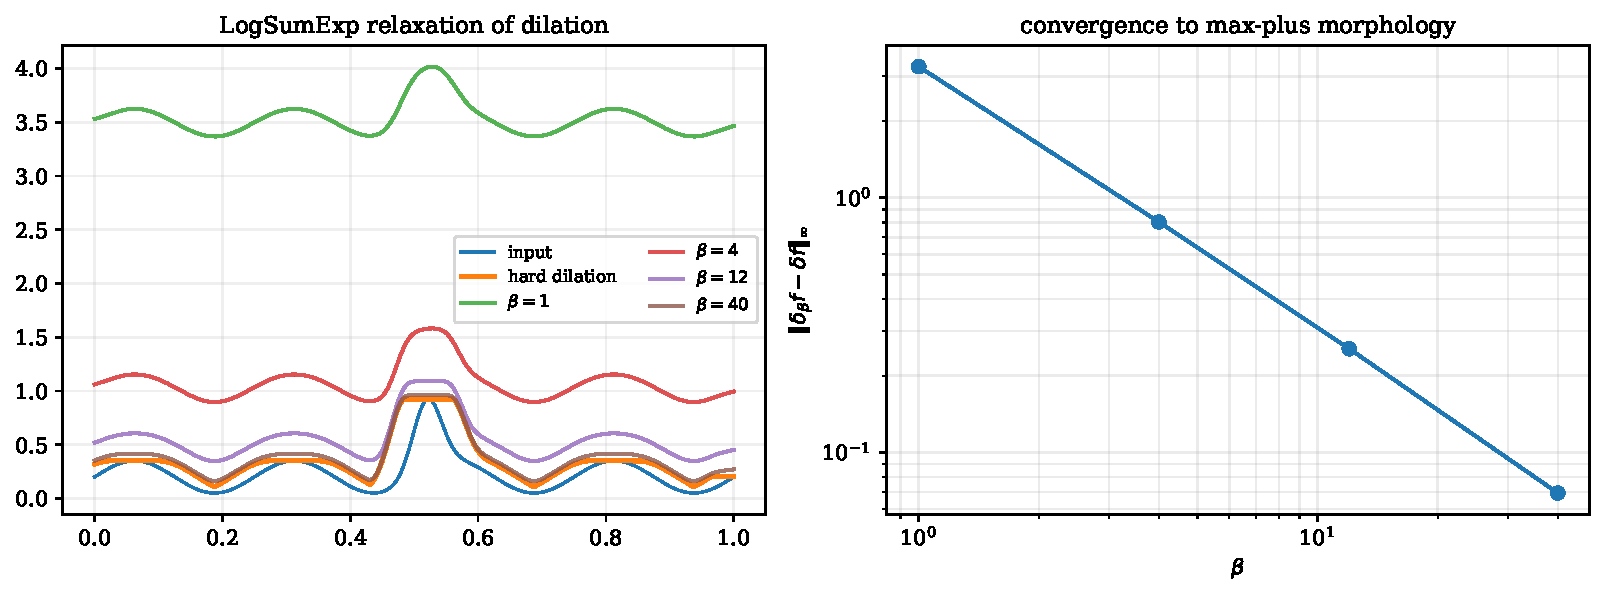
\includegraphics[width=.88\textwidth]{soft_morphology_temperature.pdf}
\caption{اثر دما بر تقریب نرم dilation و توزیع گرادیان میان اعضای پنجره.}
\end{figure}

\subsection{کران تقریب}
برای \(n\) مقدار،
\begin{equation}
\max_i z_i\le\operatorname{smax}_\tau(z)\le\max_i z_i+\tau\log n.
\end{equation}
پس دما مصالحه‌ای میان خطای تقریب و چگالی گرادیان است. annealing از دمای بزرگ به کوچک راهبرد طبیعی آموزش است.

\subsection{لایه مورفولوژیک قابل یادگیری}
یک dilation قابل یادگیری
\begin{equation}
y(p)=\max_{q\in B}\{x(p-q)+w(q)\}
\end{equation}
است. برخلاف convolution که جمع ضربی دارد، این لایه بر max-plus بنا شده و پاسخ آن به رخداد غالب محلی وابسته
است. محدودکردن \(w\)، تقارن، تنکی footprint یا پارامتری‌کردن شکل عنصر ساختاری، prior مهندسی مفیدی ایجاد می‌کند.

\section{اسکلت تفاضل‌پذیر و قیود توپولوژیک}
روش‌های soft-skeletonization با تکرار erosion نرم و استخراج باقیمانده opening، اسکلت تقریبی می‌سازند، اما
ممکن است شاخه را قطع یا حلقه کاذب ایجاد کنند. روش‌های جدیدتر تلاش می‌کنند توپولوژی را حین سازگاری با
backpropagation حفظ کنند. زیان اتصال می‌تواند بر skeleton پیش‌بینی و مرجع تعریف شود:
\begin{equation}
\mathcal L_{cl}=1-\frac{2\langle S(P),G\rangle}{\|S(P)\|_1+\|G\|_1}
+1-\frac{2\langle S(G),P\rangle}{\|S(G)\|_1+\|P\|_1}.
\end{equation}
اما این زیان جای سنجه‌های توپولوژیک مانند Betti error را نمی‌گیرد.

\section{مورفولوژی در شبکه‌های عمیق و مدل‌های بنیادی}
مورفولوژی می‌تواند در چهار سطح وارد شود: پیش‌پردازش/پس‌پردازش؛ لایه max-plus/min-plus؛ ویژگی یا پروفایل
ساختاری؛ و قید loss بر اتصال، اسکلت یا مؤلفه‌ها. برای مدل‌های بنیادی قطعه‌بندی، مورفولوژی همچنان برای تولید
prompt، پاک‌سازی mask، جداسازی اشیای چسبیده و ممیزی topology کاربرد دارد.

\begin{researchbox}
ادغام بی‌فکر opening/closing پس از شبکه ممکن است Dice را بهتر ولی topology را بدتر کند. ارزیابی باید همزمان
شامل Dice/IoU، فاصله مرزی، تعداد مؤلفه، Betti numbers، خطای مرکزخط و پایداری نسبت به رزولوشن باشد.
\end{researchbox}

\section{طراحی الگوریتم: از تعریف تا کد صحیح}
برای هر عملگر مورفولوژیک، شش تصمیم باید ثبت شود:
\begin{enumerate}
\item دامنه و نوع داده: دودویی، uint8، float یا مقدارهای بی‌نهایت؛
\item قرارداد مرز: constant، reflect، replicate یا دامنه معتبر؛
\item شکل و مرکز footprint، به‌ویژه برای اندازه زوج؛
\item اتصال پیش‌زمینه/پس‌زمینه؛
\item تفسیر پیکسل ناهمسانگرد و spacing فیزیکی؛
\item معیار صحت و پیچیدگی حافظه/زمان.
\end{enumerate}

\section{کارگاه پایتون: پیاده‌سازی‌های مرجع}
\subsection{dilation و erosion خاکستری}
\begin{latin}
\begin{lstlisting}[language=Python]
import numpy as np
from scipy.ndimage import grey_dilation, grey_erosion

def morph_gradient(image: np.ndarray, footprint: np.ndarray) -> np.ndarray:
    if image.ndim != 2 or footprint.ndim != 2:
        raise ValueError("image and footprint must be 2-D")
    dil = grey_dilation(image, footprint=footprint, mode="reflect")
    ero = grey_erosion(image, footprint=footprint, mode="reflect")
    return dil.astype(np.float64) - ero.astype(np.float64)
\end{lstlisting}
\end{latin}

\subsection{بازسازی و marker-controlled watershed}
\begin{latin}
\begin{lstlisting}[language=Python]
import numpy as np
from scipy import ndimage as ndi
from skimage import morphology, segmentation, filters

def split_touching(binary: np.ndarray) -> np.ndarray:
    binary = np.asarray(binary, dtype=bool)
    distance = ndi.distance_transform_edt(binary)
    peaks = morphology.h_maxima(distance, h=1.5)
    markers, _ = ndi.label(peaks)
    labels = segmentation.watershed(-distance, markers, mask=binary)
    return labels
\end{lstlisting}
\end{latin}

\subsection{محاسبه توپولوژی پیش و پس از پردازش}
\begin{latin}
\begin{lstlisting}[language=Python]
from skimage.measure import label, euler_number

def topology_report(mask):
    mask = mask.astype(bool)
    n4 = label(mask, connectivity=1).max()
    n8 = label(mask, connectivity=2).max()
    return {
        "components_4": int(n4),
        "components_8": int(n8),
        "euler_4": int(euler_number(mask, connectivity=1)),
        "euler_8": int(euler_number(mask, connectivity=2)),
    }
\end{lstlisting}
\end{latin}

\section{آزمایش‌های فصل}
\subsection{آزمایش ۱: اتصال و پارادوکس دیجیتال}
الگوهای قطری، حلقه و تماس نقطه‌ای بسازید و \(\beta_0,\beta_1,\chi\) را تحت زوج‌های اتصال مقایسه کنید.

\subsection{آزمایش ۲: ساختار محلی زیر نویز}
گرادیان، تانسور ساختار و هسین را در چند \(\sigma\) روی edge، corner و ridge مصنوعی با SNRهای مختلف ارزیابی کنید.

\subsection{آزمایش ۳: سرعت مورفولوژی}
پیاده‌سازی naive را با van Herk و کتابخانه برای \(k\in\{3,15,63,255\}\) مقایسه و شیب زمان نسبت به \(k\) را گزارش کنید.

\subsection{آزمایش ۴: بازسازی در برابر opening}
اشیای کشیده و لکه‌های کوچک بسازید؛ حذف نویز و اعوجاج شکل را با IoU، Hausdorff و تغییر محیط بسنجید.

\subsection{آزمایش ۵: EDT و اسکلت}
EDT تقریبی chamfer و EDT دقیق را از نظر خطا و زمان مقایسه؛ سپس حساسیت شاخه‌های اسکلت به زبری مرز را اندازه‌گیری کنید.

\subsection{آزمایش ۶: watershed نشان‌محور}
تعداد \lr{marker}، مقدار \lr{h-maxima} و میزان هموارسازی گرادیان را تغییر دهید. سپس نمودار
\lr{under-segmentation}/\lr{over-segmentation} را بسازید.

\subsection{آزمایش ۷: soft morphology}
برای دماهای مختلف، خطای تقریب max، entropy گرادیان و پایداری آموزش یک عنصر ساختاری را گزارش کنید.

\section{تمرین‌های نظری و اثباتی}
\begin{enumerate}
\item دوگانگی \((X\oplus B)^c=X^c\ominus\check B\) را اثبات کنید.
\item نشان دهید opening و closing ناشی از adjunction، idempotent هستند.
\item ثابت کنید dilation تخت نسبت به سوپریمم تصاویر توزیع‌پذیر است.
\item رابطه پاسخ تانسور ساختار با تقریب مرتبه دوم SSD وصله جابه‌جا شده را استخراج کنید.
\item کران \(\tau\log n\) برای log-sum-exp را اثبات کنید.
\item نشان دهید EDT مربع اقلیدسی در دو بعد separable است.
\item یک مثال بسازید که threshold بر ویژگی غیرافزایشی max-tree، سلسله‌مراتب را ناسازگار کند.
\item شرایطی بیابید که watershed و minimum spanning forest برچسب یکسان دهند.
\item اثر scaling رزولوشن بر compactness و طول اسکلت را تحلیل کنید.
\item یک زیان differentiable پیشنهاد دهید که هم اتصال و هم ضخامت ساختار لوله‌ای را کنترل کند.
\end{enumerate}

\section{پروژه‌های پایان فصل}
\subsection{پروژه A: آزمایشگاه مورفولوژی قابل ممیزی}
یک بسته Python بسازید که همه عملگرها را با قرارداد مرز، footprint، اتصال و آزمون خواص جبری اجرا و گزارش HTML تولید کند.

\subsection{پروژه B: قطعه‌بندی اشیای چسبیده}
خط لوله marker-controlled watershed را برای سلول، دانه یا ذرات طراحی و با روش یادگیری عمیق از نظر topology و خطای شمارش مقایسه کنید.

\subsection{پروژه C: شبکه مورفولوژیک}
یک لایه max-plus با عنصر ساختاری قابل یادگیری پیاده‌سازی، دمای softmax را anneal و شکل آموخته‌شده را تحلیل کنید.

\subsection{پروژه D: مرکزخط توپولوژی‌آگاه}
برای رگ یا جاده، segmentation و skeleton را مشترکاً آموزش دهید و Dice، clDice، Betti error و فاصله مرکزخط را گزارش کنید.

\section{پرامپت پیشنهادی برای Codex}
\begin{latin}
\begin{lstlisting}[language={}]
Build a fully reproducible Python research package for Chapter 7, "Local
Structure and Mathematical Morphology". Implement or wrap: connected-component
labeling with explicit 4/8 connectivity, Gaussian derivatives, structure tensor,
Hessian ridge measures, binary and grayscale morphology, van Herk sliding extrema,
morphological reconstruction, max-tree attribute filtering, exact Euclidean
distance transform, topology-preserving thinning, marker-controlled watershed,
granulometry, and soft differentiable morphology.

Requirements:
1. Every operator must expose border mode, footprint origin, connectivity, and
   physical pixel spacing where relevant.
2. Add property-based tests for increasingness, duality, extensivity/
   anti-extensivity, idempotence, and topology preservation.
3. Benchmark naive and optimized algorithms over image size and footprint size.
4. Produce all chapter figures and CSV tables with fixed random seeds.
5. Include synthetic cases with known ground truth and at least two real public
   images. Report accuracy, topology, runtime, and memory.
6. Implement a small PyTorch experiment that learns a soft max-plus structuring
   element with temperature annealing and compares it with convolution.
7. Never fabricate results. Save environment versions, command line arguments,
   and hashes of inputs.
\end{lstlisting}
\end{latin}

\section{تقسیم پیشنهادی ویدئوهای ۱۵ دقیقه‌ای}
\begin{longtable}{p{12mm}p{115mm}}
\toprule
بخش & موضوع \\
\midrule
1 & مسئله ساختار محلی و تفاوت زبان دیفرانسیلی و مورفولوژیک \\
2 & همسایگی، اتصال و توپولوژی دیجیتال \\
3 & CCL و union--find \\
4 & مشتق گاوسی و فضای مقیاس \\
5 & تانسور ساختار و گوشه \\
6 & هسین و ridge/vesselness \\
7 & فیلتر steerable و LBP \\
8 & مشبکه، سوپریمم و اینفیمم \\
9 & adjunction و اثبات opening/closing \\
10 & مورفولوژی دودویی \\
11 & hit-or-miss و thinning \\
12 & مورفولوژی خاکستری و max-plus \\
13 & گرادیان و top-hat \\
14 & الگوریتم van Herk \\
15 & بازسازی مورفولوژیک \\
16 & h-maxima و marker پایدار \\
17 & عملگر متصل و max-tree \\
18 & فیلتر ویژگی درختی \\
19 & تبدیل فاصله و min-convolution \\
20 & الگوریتم خطی EDT \\
21 & محور میانی و بازسازی از اسکلت \\
22 & نقطه ساده و حفظ توپولوژی \\
23 & هرس و سنجه‌های اسکلت \\
24 & watershed توپوگرافیک \\
25 & watershed گرافی و صف اولویت \\
26 & گرانولومتری و pattern spectrum \\
27 & اندازه‌گیری شکل و ممان‌ها \\
28 & پیوند مورفولوژی و PDE \\
29 & soft morphology و کران تقریب \\
30 & لایه‌های max-plus قابل یادگیری \\
31 & اسکلت تفاضل‌پذیر و قیود توپولوژیک \\
32 & کارگاه scikit-image/OpenCV \\
33 & طراحی آزمایش و ممیزی الگوریتم \\
34 & پروژه پژوهشی و مرور مرز دانش \\
\bottomrule
\end{longtable}

\section{جمع‌بندی و پل به فصل هشتم}
\begin{summarybox}
\begin{enumerate}
\item ساختار محلی با انتخاب همسایگی، مقیاس و گروه تبدیل معنا پیدا می‌کند.
\item تانسور ساختار انرژی تغییر وصله را به یک فرم درجه دوم تبدیل و لبه/گوشه را با طیف خود جدا می‌کند.
\item مورفولوژی ریاضی نظریه‌ای بر مبنای ترتیب و مشبکه است؛ dilation/erosion صرفاً فیلتر max/min نیستند.
\item adjunction منشأ خواص بنیادی opening و closing است.
\item بازسازی و عملگرهای متصل شکل اجزای باقی‌مانده را بهتر از footprint ثابت حفظ می‌کنند.
\item max-tree تصویر را به سلسله‌مراتب اجزای تراز تبدیل می‌کند و فیلتر ویژگی را کارآمد می‌سازد.
\item EDT دقیق با پوش پایین سهمی‌ها در زمان خطی محاسبه می‌شود.
\item اسکلت یک نمایش فشرده هندسه، توپولوژی و مقیاس است، اما به نویز مرز حساس است.
\item watershed بدون marker معمولاً بیش‌قطعه‌بندی می‌کند؛ کنترل مینیمم‌ها بخش اصلی الگوریتم است.
\item soft morphology امکان یادگیری می‌دهد ولی دما، خطای تقریب و جریان گرادیان باید مشترکاً تحلیل شوند.
\item در کاربردهای مدرن، Dice به تنهایی کافی نیست؛ topology، centerline و پایداری رزولوشن باید سنجیده شوند.
\item فصل بعد می‌تواند بر قطعه‌بندی و نمایش ناحیه بنا شود، زیرا اکنون ابزارهای محلی، شکلی و توپولوژیک آماده‌اند.
\end{enumerate}
\end{summarybox}

\backmatter
\chapter*{منابع منتخب فصل}
\addcontentsline{toc}{chapter}{منابع منتخب فصل}
\begin{latin}
\begin{thebibliography}{99}
\bibitem{serra1982} J. Serra, \textit{Image Analysis and Mathematical Morphology}, Academic Press, 1982.
\bibitem{soille2003} P. Soille, \textit{Morphological Image Analysis}, 2nd ed., Springer, 2003.
\bibitem{najman2013} L. Najman and H. Talbot, eds., \textit{Mathematical Morphology: From Theory to Applications}, Wiley, 2013.
\bibitem{heijmans1994} H. J. A. M. Heijmans, \textit{Morphological Image Operators}, Academic Press, 1994.
\bibitem{matheron1975} G. Matheron, \textit{Random Sets and Integral Geometry}, Wiley, 1975.
\bibitem{lindeberg1994} T. Lindeberg, \textit{Scale-Space Theory in Computer Vision}, Springer, 1994.
\bibitem{harris1988} C. Harris and M. Stephens, ``A combined corner and edge detector,'' Alvey Vision Conference, 1988.
\bibitem{shi1994} J. Shi and C. Tomasi, ``Good features to track,'' CVPR, 1994.
\bibitem{frangi1998} A. F. Frangi et al., ``Multiscale vessel enhancement filtering,'' MICCAI, 1998.
\bibitem{ojala2002} T. Ojala, M. Pietikäinen, and T. Mäenpää, ``Multiresolution gray-scale and rotation invariant texture classification with local binary patterns,'' TPAMI, 2002.
\bibitem{vanherk1992} M. van Herk, ``A fast algorithm for local minimum and maximum filters on rectangular and octagonal kernels,'' Pattern Recognition Letters, 1992.
\bibitem{gilwerman1993} J. Gil and M. Werman, ``Computing 2-D min, median, and max filters,'' TPAMI, 1993.
\bibitem{vincent1993} L. Vincent, ``Morphological grayscale reconstruction in image analysis: Applications and efficient algorithms,'' TIP, 1993.
\bibitem{salembier1998} P. Salembier, A. Oliveras, and L. Garrido, ``Antiextensive connected operators for image and sequence processing,'' TIP, 1998.
\bibitem{najman2006} L. Najman and M. Couprie, ``Building the component tree in quasi-linear time,'' TIP, 2006.
\bibitem{carlinet2014} E. Carlinet and T. Géraud, ``A comparative review of component tree computation algorithms,'' TIP, 2014.
\bibitem{passat2023} N. Passat and B. Naegel, ``Morphological hierarchies: A unifying framework with new perspectives,'' 2023.
\bibitem{felzenszwalb2012} P. F. Felzenszwalb and D. P. Huttenlocher, ``Distance transforms of sampled functions,'' Theory of Computing, 2012.
\bibitem{zhang1984} T. Y. Zhang and C. Y. Suen, ``A fast parallel algorithm for thinning digital patterns,'' CACM, 1984.
\bibitem{lee1994} T.-C. Lee, R. L. Kashyap, and C.-N. Chu, ``Building skeleton models via 3-D medial surface/axis thinning algorithms,'' CVGIP, 1994.
\bibitem{meyer1994} F. Meyer, ``Topographic distance and watershed lines,'' Signal Processing, 1994.
\bibitem{couprie2011} C. Couprie, L. Grady, L. Najman, and H. Talbot, ``Power watershed: A unifying graph-based optimization framework,'' TPAMI, 2011.
\bibitem{shih2019} Y. Shen, X. Zhong, and F. Y. Shih, ``Deep morphological neural networks,'' arXiv:1909.01532, 2019.
\bibitem{angulo2021} J. Angulo, ``Some open questions on morphological operators and representations in the deep learning era,'' 2021.
\bibitem{hu2021} Y. Hu et al., ``Learning deep morphological networks with neural architecture search,'' 2021.
\bibitem{blusseau2024} S. Blusseau, ``Training morphological neural networks with gradient descent: Some theoretical insights,'' 2024.
\bibitem{menten2023} M. J. Menten et al., ``A skeletonization algorithm for gradient-based optimization,'' ICCV, 2023.
\bibitem{shit2021} S. Shit et al., ``clDice: A novel topology-preserving loss function for tubular structure segmentation,'' CVPR, 2021.
\bibitem{shamsi2024} A. Shamsi et al., ``Improved topological preservation in 3D axon segmentation and centerline detection,'' WACV, 2024.
\bibitem{forte2025} J. M. Forte et al., ``Consistent connected operators based on trees of shapes,'' SIAM Journal on Imaging Sciences, 2025.
\bibitem{skimage2026} scikit-image Developers, ``Morphology API: max-tree, reconstruction, skeletonize, medial axis and area operators,'' documentation, accessed 2026.
\bibitem{opencv2026} OpenCV Development Team, ``Morphological transformations, distance transform and watershed,'' documentation, accessed 2026.
\end{thebibliography}
\end{latin}

\chapter*{راهنمای کامپایل، فونت و اجرای آزمایش‌ها}
\addcontentsline{toc}{chapter}{راهنمای کامپایل، فونت و اجرای آزمایش‌ها}
فایل با \lr{XeLaTeX} کامپایل می‌شود. فونت اصلی \lr{Amiri}، فونت لاتین \lr{DejaVu Serif} و فونت کد
\lr{DejaVu Sans Mono} است و برای هر سه جایگزین خودکار تعریف شده است. فایل فونت در بسته توزیع نمی‌شود.

\begin{latin}
\begin{lstlisting}[language=bash]
python -m venv .venv
# Windows: .venv\Scripts\activate
# Linux/macOS: source .venv/bin/activate
pip install -r requirements.txt
python generate_figures.py
xelatex image_processing_next_decade_ch07_fa.tex
xelatex image_processing_next_decade_ch07_fa.tex
\end{lstlisting}
\end{latin}
\end{document}
